\documentclass[dvipsnames,svgnames]{beamer}
\usetheme{Warsaw}
\usepackage[utf8]{inputenc}
\usepackage[english]{babel}
\usepackage{amsmath}
\usepackage{amsfonts}
\usepackage{amssymb}
\usepackage{graphicx}
\usepackage[linesnumbered,ruled]{algorithm2e}
\usepackage{tikz}
\usetikzlibrary{automata, positioning}
\usepackage{float}
\usepackage[normalem]{ulem}
\usepackage{color}
\usepackage{xcolor}

\expandafter\def\expandafter\insertshorttitle\expandafter{%
	\insertshorttitle\hfill%
    \insertframenumber\,/\,\inserttotalframenumber}



\author{Charles Dufour}
\title{Reinforcement learning and robot navigation }
%\setbeamercovered{transparent} 
\setbeamertemplate{navigation symbols}{} 
%\logo{} 
%\institute{} 
\date{May 2, 2018}
%\subject{} 

\newtheorem{madef}{Definition}

\begin{document}


\begin{frame}
\titlepage
\centering
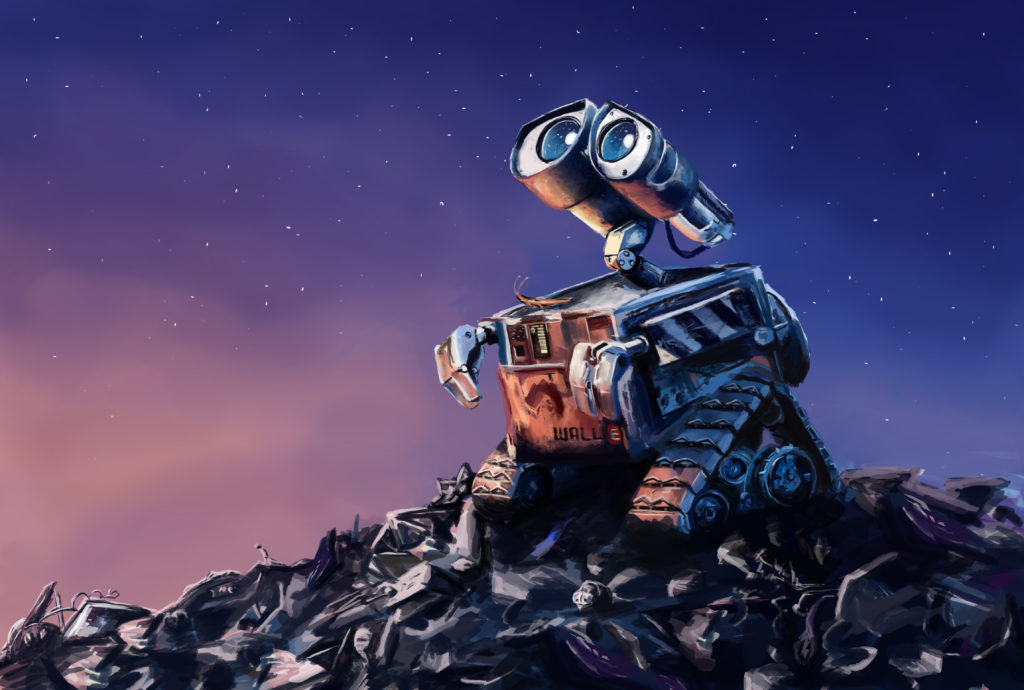
\includegraphics[scale=1]{img/Wall-E.jpg}
\end{frame}

%\begin{frame}
%\tableofcontents
%\end{frame}



\begin{frame}
\frametitle{Introduction}
\begin{block}{The problem}

  \begin{itemize}
   \item Framework: a raspberry pie 3 robot which can follow lines
   \item The task: the robot should adapt its speed with respect to traffic lights
   \item How: using Reinforcement Learning (RL) and Markov Decision Process (MDP)  
  \end{itemize}
\end{block} 
\end{frame}

\begin{frame}
\frametitle{The task}
\begin{center}
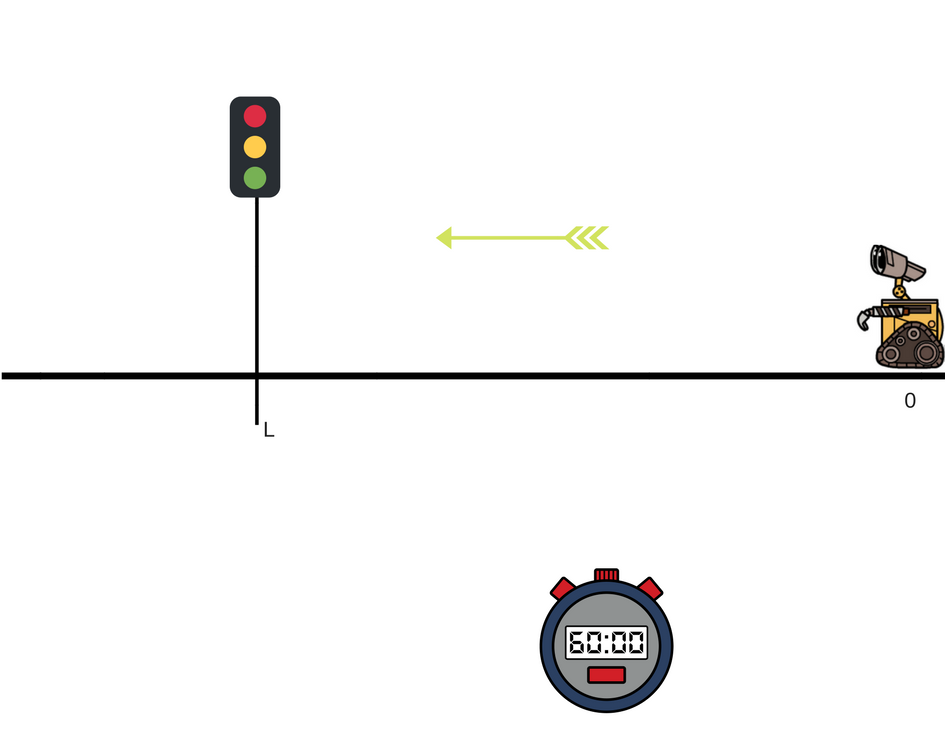
\includegraphics[scale=0.4]{img/illustration_traffic_light.png}
\end{center}
\end{frame}

\begin{frame}{Presentation}
\begin{block}{}
\begin{itemize}
\item Part I: theoretical background 
\item Part II: results from first implementations
\end{itemize}
\end{block}
\end{frame}

\begin{frame}
\frametitle{Reinforcement learning}
\centering
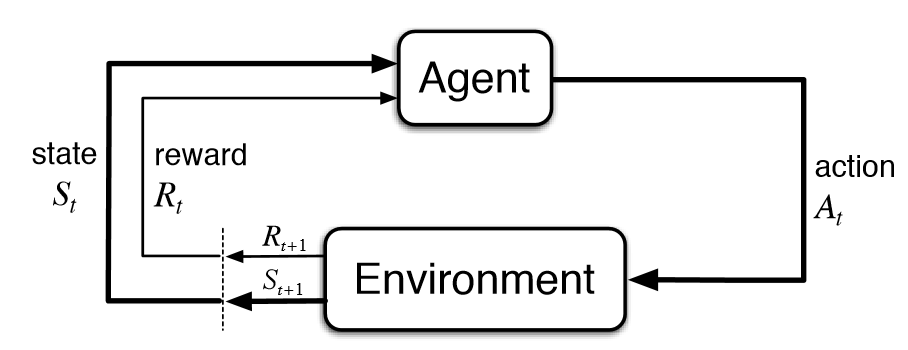
\includegraphics[scale=0.5]{img/RL_graph.png}
\vspace{1cm}

The agent's job is to find a behavior that maximizes the long-run sum of values of the rewards.
\end{frame}

\begin{frame}
\frametitle{Markov Decision Process intuition}

\begin{figure}[ht]
\centering
    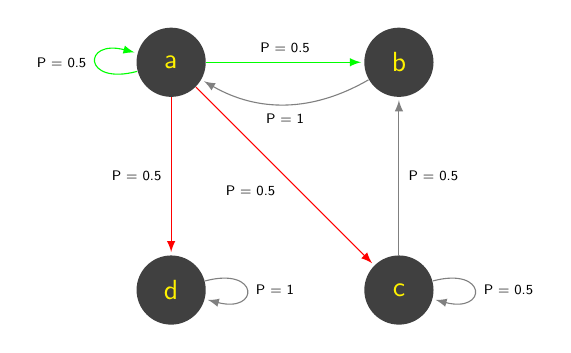
\begin{tikzpicture}[font=\sffamily]
    % Add the states
        \node[state,
              text=yellow,
              draw=none,
              fill=gray!50!black] (0) {a};
        \node[state,
              right=2cm of 0,
              text=yellow,
              draw=none, 
              fill=gray!50!black] (1) {b};
        \node[state,
              below=2cm of 1,
              text=yellow,
              draw=none, 
              fill=gray!50!black] (2) {c};
        \node[state,
        	  below = 2cm of 0,
        	  text=yellow,
        	  draw=none,
        	  fill=gray!50!black] (3) {d};
     

              
 \draw[every loop,
        auto=right,
        >=latex,
        draw=gray,
        fill=gray]
        
        	(0) edge[loop left, draw = green] node {{\tiny P = 0.5}}(0)
        	(0) edge[ auto = right,draw = red]  node {{\tiny P = 0.5}}(2)
        	(0) edge[auto = right,draw = red] node{{\tiny P = 0.5}}  (3)
            (0) edge[auto = left,draw=green]  node {{\tiny P = 0.5}} (1)
            (1) edge[bend left,auto =left]  node {{\tiny P = 1}} (0)
            (2) edge[]  node {{\tiny P = 0.5}}(1)
			(2) edge[loop right] node{{\tiny P = 0.5}} (2)
			(3) edge[loop right] node{{\tiny P = 1}} (3)	
			       
            ;       
      
    \end{tikzpicture}

\end{figure}
actions possible in state 0:
\begin{enumerate}

\item \textcolor{green}{$\rightarrow$}: action 1
\item \textcolor{red}{$\rightarrow$}: action 2

\end{enumerate}


Episode : $s_0; a_1,s_1,r_1; a_2,s_2,r_2; \ldots; a_{n},s_{n},r_{n}$

\end{frame}






\begin{frame}
\frametitle{Markov Decision Process}
\begin{block}{Definition: (MDP) }
\begin{itemize}
\item A set of states $\mathcal{S}=\{s_0,s_1,s_2,\ldots,s_{n}\}$
\item A set of actions $\mathcal{A}=\{a_1,a_2,a_3,\ldots,a_{k}\}$
\item A transition function $T(a,s,s') = \mathbb{P}[s'\mid a,s]$
\item A reward function $R: \mathcal{S}\mapsto \mathbb{R}$
\item A discount factor $0 \leq \gamma < 1$ 
\end{itemize}
\end{block}

\begin{block}{Markov property}
The transitions only depends on the current state and the current action.
\end{block}
\end{frame}

%\begin{frame}
%\frametitle{to be told}
%Particularly, at each time step, our process is in some state $s$.\\Then our learning agent decides which action to execute from the set $\mathcal{A}$ which is doable from state $s$.\\Then the process moves randomly to a new state $s'$ following $T$ and gives the agent a reward $R(s')$.\\The purpose of our agent is to maximise the cumulative reward it gets in the long run.
%
%\end{frame}





\begin{frame}
\frametitle{How to pick actions}
\begin{block}{Definition: (policy)}
A \emph{policy} $\pi$ is a probabilistic mapping from the set of states to the set of actions : 
$$ \pi : \mathcal{A} x \mathcal{S} \mapsto [0,1] $$
\\
s.t. $\underset{a}{\sum } \pi(a\mid s)=1 \quad \forall s \in \mathcal{S}$

\end{block}
\end{frame}

\begin{frame}
\frametitle{Issue}
\begin{alertblock}{How to}
How to asses the quality of policies so we can find the best one? 

What is the best policy?
\end{alertblock}
\end{frame}

\begin{frame}
\frametitle{How to asses the quality of policies}
\begin{block}{We are interested in maximizing the discounted return: $G_t$}
$$ G_t= \sum_{k=0}^{\infty}\gamma^k R_{t+k+1} = R_{t+1} + \gamma G_{t+1}$$
\end{block}

\pause
\begin{block}{Action value while in a state s under $\pi$}
\begin{equation*}
q_{\pi}(s,a) = \mathbb{E}_{\pi}[G_t\mid S_t =s,A_t=a]
\end{equation*}
\end{block}

\pause
\begin{block}{State value under policy $\pi$}
\begin{equation*}
v_{\pi}(s)=\mathbb{E}_{\pi}[G_t \mid S_t=s]
\end{equation*}
\end{block}



\end{frame}

\begin{frame}
\frametitle{Recursive definition of value functions}
\begin{block}{action value}
\begin{equation*}
q_{\pi}(s,a) =  \sum_{s'}\mathbb{P}(s'\mid a,s)\left[R(s') + \gamma v_{\pi}(s') \right]
\end{equation*}
\end{block}

\begin{block}{state value}
\begin{equation*}
v_{\pi}(s) =\sum_{a }\pi(a \mid s) \sum_{s'}\mathbb{P}(s'\mid a,s)\left[R(s') + \gamma v_{\pi}(s') \right]
\end{equation*}
\end{block}
\end{frame}

%\begin{frame}
%\frametitle{Recursive definition of value functions}
%\begin{block}{action value}
%\begin{equation*}
%\begin{split}
%q_{\pi}(s,a) &= \mathbb{E}_{\pi}[G_t\mid S_t =s, A_t=a]
%\\&=\mathbb{E}_{\pi}[R_{t+1}+\gamma G_{t+1}\mid S_t =s, A_t=a]
%\\& =\sum_{s'}\mathbb{P}(s'\mid a,s)\left[r + \gamma \mathbb{E}_{\pi}\left[G_{t+1} \mid S_{t+1}=s' \right]\right]
%\\& = \sum_{s'}\mathbb{P}(s'\mid a,s)\left[r + \gamma v_{\pi}(s') \right]
%\end{split}
%\end{equation*}
%\end{block}
%
%with $r=R(s')$
%\end{frame}


%\begin{frame}
%\frametitle{Recursive definition of value functions}
%\begin{block}{state value}
%\begin{equation*}
%\begin{split}
%v_{\pi}(s) &= \mathbb{E}_{\pi}[G_t\mid S_t =s]
%\\&=\mathbb{E}_{\pi}[R_{t+1}+\gamma G_{t+1}\mid S_t =s]
%\\& =\sum_{a }\pi(a \mid s) \sum_{s'}\mathbb{P}(s'\mid a,s)\left[r + \gamma \mathbb{E}_{\pi}\left[G_{t+1} \mid S_{t+1}=s' \right]\right]
%\\& =\sum_{a }\pi(a \mid s) \sum_{s'}\mathbb{P}(s'\mid a,s)\left[r + \gamma v_{\pi}(s') \right]
%\\&=\sum_{a }\pi(a \mid s)q_{\pi}(s,a)
%\end{split}
%\end{equation*}
%\end{block}
%
%with $r=R(s')$
%\end{frame}




\begin{frame}
\frametitle{How to asses the quality of policies}
\begin{block}{How to compare two policies}
$$ \pi \leq \pi ' \iff  v_{\pi}(s) \leq v_{\pi'}(s) \quad \forall s \in \mathcal{S}
$$
\end{block}

\pause 

\begin{block}{Optimal policy}
$$ \pi_{*} \quad s.t. \quad \forall \pi : \pi_{*}\geq \pi $$
\end{block}
\end{frame}

%\begin{frame}
%\frametitle{Bellman optimality principle}
% An optimal policy has the property that whatever the initial state and initial decision are, the remaining decisions must constitute an optimal policy with regard to the state resulting from the first decision. (See Bellman, 1957, Chap. III.3.)
%\end{frame}

\begin{frame}
\frametitle{Bellman optimality equations}

We can associate the value function $v_*$ and $q_*$ to the optimal policy $\pi_{*}$   

\begin{block}{}

\begin{equation*}
v_{*}(s)=\underset{a}{\text{max }} q_{*}(s,a)
\end{equation*}
\end{block}

\begin{block}{}
\begin{equation*}
\begin{split}
q_{*}(s,a) = \sum_{s'}\mathbb{P}(s' \mid s,a)[R(s')+\gamma \max_{a'}q_{*}(s',a')]
\end{split}
\end{equation*}
\end{block}

%Intuitively these equations say that the value of a state under the optimal policy must equal the expected return for the best action from that state. For finite MDPs these equations have a unique solution.
\end{frame}


\begin{frame}
\frametitle{Finding optimal policy from value functions}
\begin{block}{}

$$\pi_{*}(s)= \underset{a}{\text{argmax }}q_*(s,a)$$
\end{block}
\end{frame}

\begin{frame}
\frametitle{Another issue}
\begin{alertblock}{Computational issue}
$\mid \mathcal{S} \mid $ linear equations to solve to evaluate policy\\
%\begin{center}
% $O(\mid \mathcal{S} \mid ^2)$
% \end{center}
$\mid \mathcal{S} \mid $ non linear equations to solve the Bellman optimality equation 
%\begin{center}
%$O(\mid \mathcal{S} \mid ^3)$ blablablabla
%\end{center}
\end{alertblock}

\pause 
\vspace{1cm}
\centering
Approximation of value function
\\ and
\\Policy iteration

\end{frame}

%\begin{frame}
%\frametitle{Solving MDP using dynamic programming}
%\begin{block}{iterative policy evaluation}
%update rule : 
%$$ v_{k+1}(s)=\sum_{a \in \mathcal{A}}\pi(a \mid s)\sum_{s'}T(a,s,s')\left[R(s')+\gamma v_k(s')\right] $$
%\end{block}
%\pause
%\begin{block}{policy improvement}
%$\pi/\pi'$ : old/new policy.
%$$\pi'(s) = \underset{a \in \mathcal{A}}{\text{argmax } } q_{\pi}(s,a) $$
%\end{block}
%
%\end{frame}


\begin{frame}
\frametitle{Policy iteration algorithm}
\framesubtitle{solving MDP using dynamic programming }
%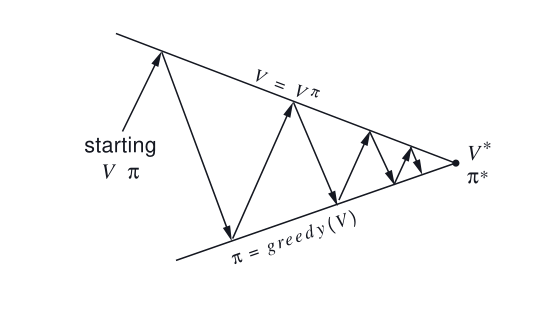
\includegraphics[scale=0.6]{img/generalized_policy_iter_sutton.png}
\centering
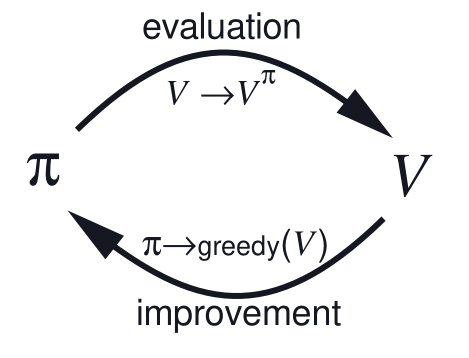
\includegraphics[scale=0.7]{img/policy_iter_sutton.PNG}
\footnote{From (Sutton \& Barto, 1998)}
\end{frame}


%\begin{frame}
%\frametitle{Monte-Carlo methods}
%\framesubtitle{model-free methods}
%\begin{block}{Idea}
%\begin{itemize}
%\item evaluates action value 
%\item improves the policy greedily (as before)
%\item learns from experience by averaging the reward received in episodes
%\end{itemize}
%\end{block}
%\end{frame}
%
%\begin{frame}
%\frametitle{One last algorithm: Q-learning}
%\framesubtitle{model-free algorithms}
%\begin{block}{Update rule}
%\begin{equation*}
%\centering
%Q(S_t,A_t) \leftarrow Q(S_t,A_t)+\alpha \left[ R_{t+1} + \gamma \max_{a}Q(S_{t+1},a)-Q(S_t,A_t) \right]
%\end{equation*}
%\end{block}
%\pause
%\begin{block}{Properties}
%\begin{itemize}
%\item learns from raw experience without a model if the environment
%\item does not wait for the end of the episode to update the state value actions
%\item approximation of the optimal action values not the states values
%\item can be shown to converge quadratically as the number of visits of the  pairs state-action approaches infinity
%\end{itemize}
%\end{block}
%\end{frame}

\begin{frame}
\frametitle{Our problem}
\begin{center}
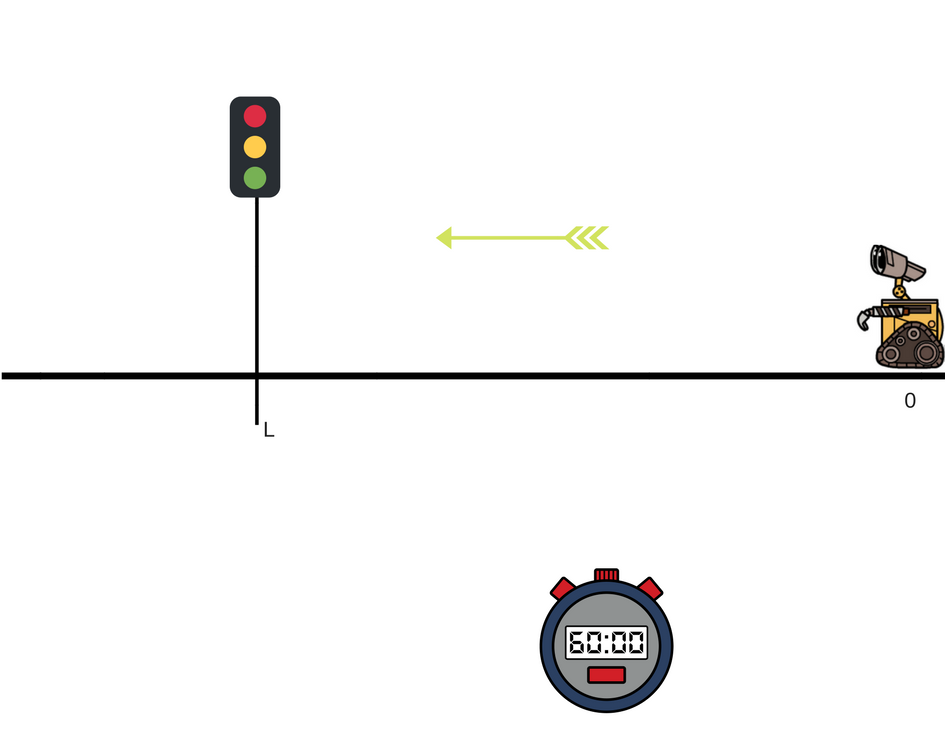
\includegraphics[scale=0.4]{img/illustration_traffic_light.png}
\end{center}
\end{frame}


\begin{frame}
\frametitle{First a simpler problem}
\begin{center}
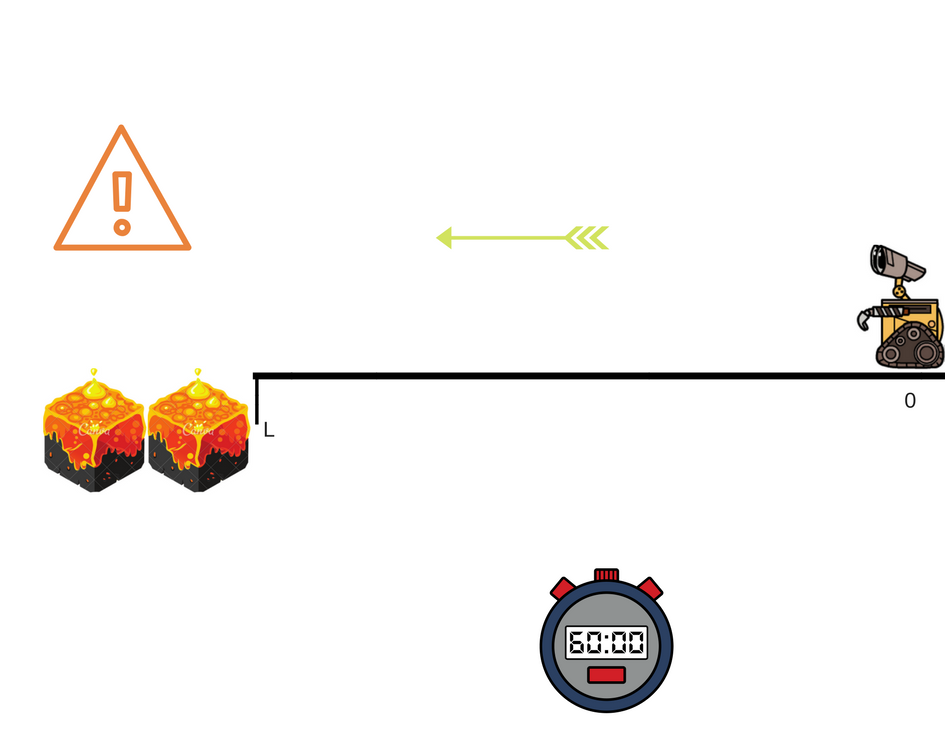
\includegraphics[scale=0.4]{img/illustration_lava.png}
\end{center}
\end{frame}

\begin{frame}
\frametitle{Modelization}
\begin{block}{states}
\begin{itemize}
\item  position \{0,1,2,\ldots ,L, Lava  \}
\item  speed    \{low, medium, high   \}
\end{itemize}
\end{block}
\pause
\begin{block}{actions}
\begin{itemize}
\item  slowing down
\item  maintaining speed
\item  speeding up 
\end{itemize}
\end{block}
\pause
\begin{block}{reward function}
\begin{itemize}
\item Lava: reward of -L
\item L in low speed: reward of +L
\item any other state : reward of -1
\end{itemize}
\end{block}

\end{frame}


\begin{frame}
\begin{center}
\frametitle{Maintaining speed}

\begin{tikzpicture}[font=\sffamily]
    % Add the states
        %\node[state,draw=none] (d1) [left of=1] {};
        \node[state,draw = none
              ] (h0) {};
		\node[state,
			below=1 cm of h0,
        	draw=none
        	] (m0) {};
		\node[state,
			below= 1 cm of m0,
        	text=black,
        	] (l0) {0};
         \node[state,
         	 right = 1 cm of h0,
             draw=none
              ] (h1) {};	
		\node[state,
			below=1 cm of h1,
        	draw = none
        	] (m1) {};
		\node[state,
			below= 1 cm of m1,
        	text=black,
        	] (l1) {1};
         \node[state,
         	right = 1 cm of h1,
              draw = none
              ] (h2) {};	
		\node[state,
			below=1 cm of h2,
        	draw = none,
        	] (m2) {};
		\node[state,
		below= 1 cm of m2,
        	text=black,
        	] (l2) {2};
        \node[state,
        	right = 1 cm of h2,
        	draw = none
             ] (h3) {};	
		\node[state,
			below=1 cm of h3,
        	draw = none
        	] (m3) {};
		\node[state,
			below= 1 cm of m3,
        	text=black,
        	] (l3) {3};   	
		\node[state,draw=none] (d1) [right = 1 cm of l3] {};	
		\node[draw=none] (legend1) [left=0.3 cm of l0] {low speed};
		        
       \draw[every loop,
        auto=right,
        >=latex,
        draw=blue,
        fill=blue]
			(l0) edge[](l1)
			(l1) edge[] (l2)	
			(l2) edge[] (l3)
			(l3) edge[dashed] (d1)
			
	       
            ;
    \end{tikzpicture}
    
     \end{center}



\end{frame}

\begin{frame}
\begin{center}
\frametitle{Maintaining speed}

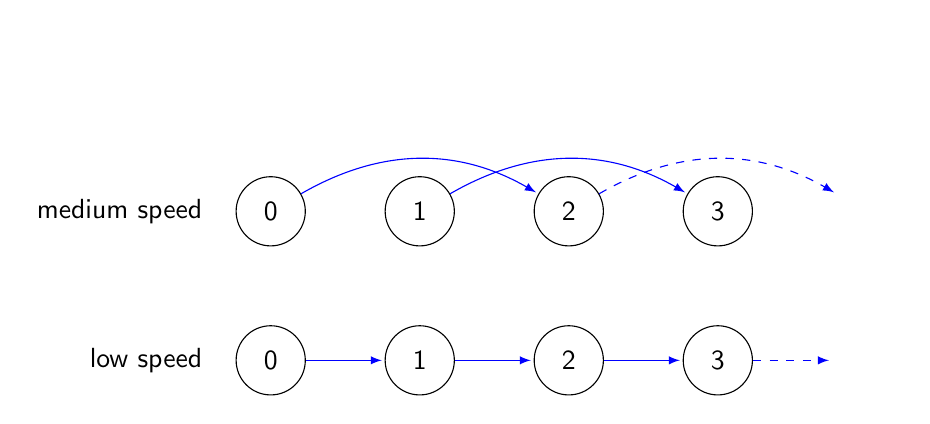
\begin{tikzpicture}[font=\sffamily]
    % Add the states
        %\node[state,draw=none] (d1) [left of=1] {};
        \node[state,draw = none
              ] (h0) {};
		\node[state,
			below=1 cm of h0,
			text = black
        	] (m0) {0};
		\node[state,
			below= 1 cm of m0,
        	text=black,
        	] (l0) {0};
         \node[state,
         	 right = 1 cm of h0,
             draw=none
              ] (h1) {};	
		\node[state,
			below=1 cm of h1,
        	text = black
        	] (m1) {1};
		\node[state,
			below= 1 cm of m1,
        	text=black,
        	] (l1) {1};
         \node[state,
         	right = 1 cm of h1,
              draw = none
              ] (h2) {};	
		\node[state,
			below=1 cm of h2,
        	text = black,
        	] (m2) {2};
		\node[state,
		below= 1 cm of m2,
        	text=black,
        	] (l2) {2};
        \node[state,
        	right = 1 cm of h2,
        	draw = none
             ] (h3) {};	
		\node[state,
			below=1 cm of h3,
        	text=black
        	] (m3) {3};
		\node[state,
			below= 1 cm of m3,
        	text=black,
        	] (l3) {3};   	
		\node[state,draw=none] (d1) [right = 1 cm of l3] {};	
		\node[state,draw=none] (d2) [right = 1 cm of m3] {};
		\node[state,draw=none] (d3) [right = 1 cm of h3] {};
		\node[draw=none] (legend1) [left=0.3 cm of l0] {low speed};
		\node[draw=none] (legend2) [left = 0.3 cm of m0] {\textcolor{black}{medium speed}};
		        
       \draw[every loop,
        auto=right,
        >=latex,
        draw=blue,
        fill=blue]
			(l0) edge[](l1)
			(l1) edge[] (l2)	
			(l2) edge[] (l3)
			(l3) edge[dashed] (d1)
			(m0) edge[bend left] (m2)
			(m1) edge[bend left] (m3)
			(m2) edge[bend left,dashed] (d2)
			
	       
            ;
    \end{tikzpicture}
     \end{center}



\end{frame}


\begin{frame}
\begin{center}
\frametitle{Maintaining speed}

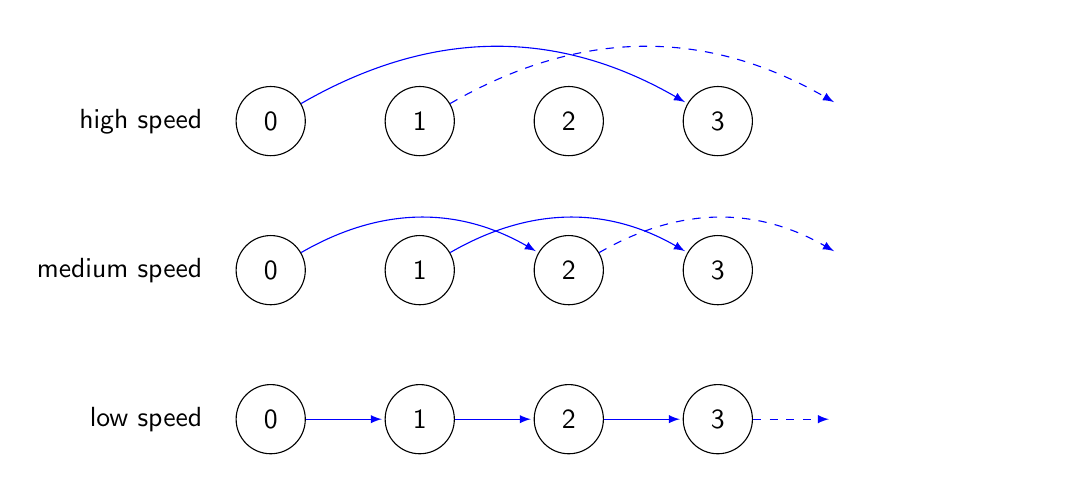
\begin{tikzpicture}[font=\sffamily]
    % Add the states
        %\node[state,draw=none] (d1) [left of=1] {};
        \node[state,text = black
              ] (h0) {0};
		\node[state,
			below=1 cm of h0,
			text = black
        	] (m0) {0};
		\node[state,
			below= 1 cm of m0,
        	text=black,
        	] (l0) {0};
         \node[state,
         	 right = 1 cm of h0,
             text = black
              ] (h1) {1};	
		\node[state,
			below=1 cm of h1,
        	text = black
        	] (m1) {1};
		\node[state,
			below= 1 cm of m1,
        	text=black,
        	] (l1) {1};
         \node[state,
         	right = 1 cm of h1,
         	text = black
              ] (h2) {2};	
		\node[state,
			below=1 cm of h2,
        	text = black,
        	] (m2) {2};
		\node[state,
		below= 1 cm of m2,
        	text=black,
        	] (l2) {2};
        \node[state,
        	right = 1 cm of h2,
        	text = black
             ] (h3) {3};	
		\node[state,
			below=1 cm of h3,
        	text=black
        	] (m3) {3};
		\node[state,
			below= 1 cm of m3,
        	text=black,
        	] (l3) {3};   	
		\node[state,draw=none] (d1) [right = 1 cm of l3] {};	
		\node[state,draw=none] (d2) [right = 1 cm of m3] {};
		\node[state,draw=none] (d3) [right = 1 cm of h3] {};
		\node[state,draw=none] (d4) [right = 1 cm of d3] {};
		\node[draw=none] (legend1) [left=0.3 cm of l0] {low speed};
		\node[draw=none] (legend2) [left = 0.3 cm of m0] {\textcolor{black}{medium speed}};
		\node[draw=none] (legend3) [left = 0.3 cm of h0] {\textcolor{black}{high speed}};
		        
       \draw[every loop,
        auto=right,
        >=latex,
        draw=blue,
        fill=blue]
			(l0) edge[](l1)
			(l1) edge[] (l2)	
			(l2) edge[] (l3)
			(l3) edge[dashed] (d1)
			(m0) edge[bend left] (m2)
			(m1) edge[bend left] (m3)
			(m2) edge[bend left,dashed] (d2)
			(h0) edge[bend left] (h3)
			(h1) edge[bend left,dashed] (d3)
			
	       
            ;
    \end{tikzpicture}
     \end{center}



\end{frame}




\begin{frame}
\begin{center}
\frametitle{Speeding up}
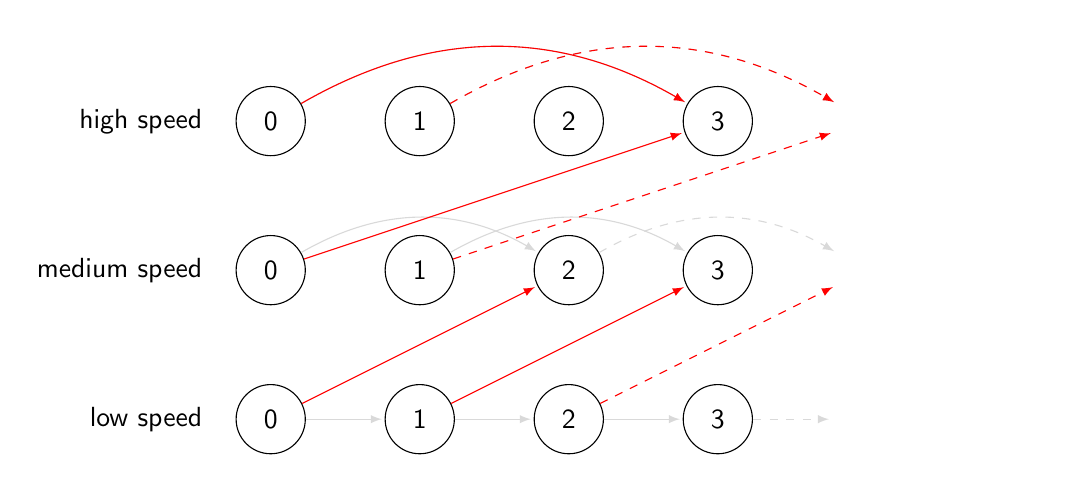
\begin{tikzpicture}[font=\sffamily]
    % Add the states
        %\node[state,draw=none] (d1) [left of=1] {};
        \node[state,text = black
              ] (h0) {0};
		\node[state,
			below=1 cm of h0,
			text = black
        	] (m0) {0};
		\node[state,
			below= 1 cm of m0,
        	text=black,
        	] (l0) {0};
         \node[state,
         	 right = 1 cm of h0,
             text = black
              ] (h1) {1};	
		\node[state,
			below=1 cm of h1,
        	text = black
        	] (m1) {1};
		\node[state,
			below= 1 cm of m1,
        	text=black,
        	] (l1) {1};
         \node[state,
         	right = 1 cm of h1,
         	text = black
              ] (h2) {2};	
		\node[state,
			below=1 cm of h2,
        	text = black,
        	] (m2) {2};
		\node[state,
		below= 1 cm of m2,
        	text=black,
        	] (l2) {2};
        \node[state,
        	right = 1 cm of h2,
        	text = black
             ] (h3) {3};	
		\node[state,
			below=1 cm of h3,
        	text=black
        	] (m3) {3};
		\node[state,
			below= 1 cm of m3,
        	text=black,
        	] (l3) {3};   	
		\node[state,draw=none] (d1) [right = 1 cm of l3] {};	
		\node[state,draw=none] (d2) [right = 1 cm of m3] {};
		\node[state,draw=none] (d3) [right = 1 cm of h3] {};
		\node[state,draw=none] (d4) [right = 1 cm of d3] {};
		\node[draw=none] (legend1) [left=0.3 cm of l0] {low speed};
		\node[draw=none] (legend2) [left = 0.3 cm of m0] {\textcolor{black}{medium speed}};
		\node[draw=none] (legend3) [left = 0.3 cm of h0] {\textcolor{black}{high speed}};
		        
       \draw[every loop,
        auto=right,
        >=latex,
        draw=gray!30,
        fill=gray!30]
			(l0) edge[](l1)
			(l1) edge[] (l2)	
			(l2) edge[] (l3)
			(l3) edge[dashed] (d1)
			(m0) edge[bend left] (m2)
			(m1) edge[bend left] (m3)
			(m2) edge[bend left,dashed] (d2)
			(h0) edge[bend left] (h3)
			(h1) edge[bend left,dashed] (d3)
            ;
      \draw[every loop,
        auto=right,
        >=latex,
        draw=red,
        fill=red]
			(l0) edge[](m2)
			(l1) edge[] (m3)	
			(m0) edge[] (h3)
			(h0) edge[bend left] (h3)
			(h1) edge[bend left,dashed] (d3)
			(l2) edge[dashed] (d2)
			(m1) edge[dashed] (d3);
    \end{tikzpicture}
     \end{center}



\end{frame}
		        



\begin{frame}
\begin{center}
\frametitle{Slowing down}

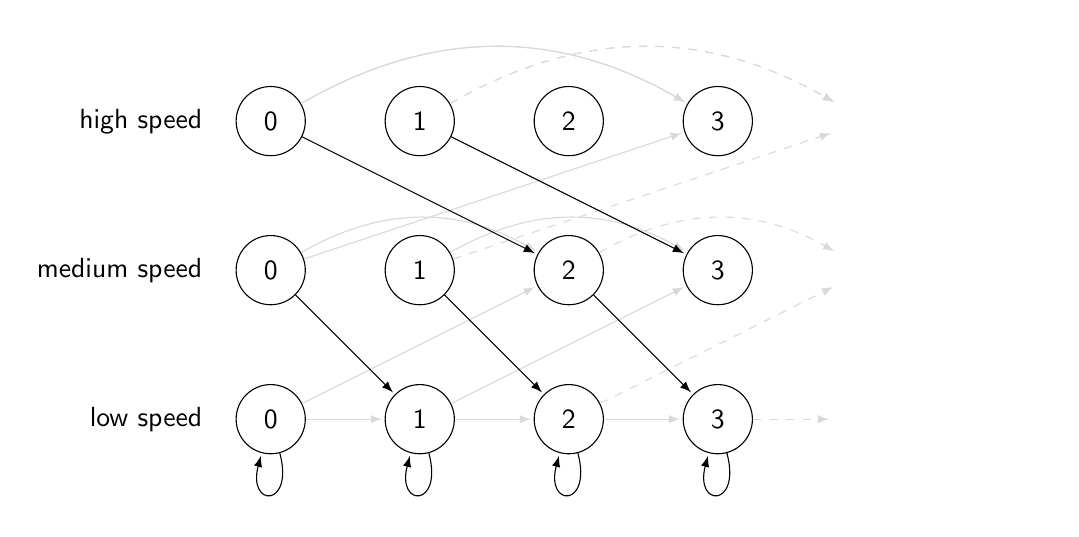
\begin{tikzpicture}[font=\sffamily]
    % Add the states
        %\node[state,draw=none] (d1) [left of=1] {};
        \node[state,text = black
              ] (h0) {0};
		\node[state,
			below=1 cm of h0,
			text = black
        	] (m0) {0};
		\node[state,
			below= 1 cm of m0,
        	text=black,
        	] (l0) {0};
         \node[state,
         	 right = 1 cm of h0,
             text = black
              ] (h1) {1};	
		\node[state,
			below=1 cm of h1,
        	text = black
        	] (m1) {1};
		\node[state,
			below= 1 cm of m1,
        	text=black,
        	] (l1) {1};
         \node[state,
         	right = 1 cm of h1,
         	text = black
              ] (h2) {2};	
		\node[state,
			below=1 cm of h2,
        	text = black,
        	] (m2) {2};
		\node[state,
		below= 1 cm of m2,
        	text=black,
        	] (l2) {2};
        \node[state,
        	right = 1 cm of h2,
        	text = black
             ] (h3) {3};	
		\node[state,
			below=1 cm of h3,
        	text=black
        	] (m3) {3};
		\node[state,
			below= 1 cm of m3,
        	text=black,
        	] (l3) {3};   	
		\node[state,draw=none] (d1) [right = 1 cm of l3] {};	
		\node[state,draw=none] (d2) [right = 1 cm of m3] {};
		\node[state,draw=none] (d3) [right = 1 cm of h3] {};
		\node[state,draw=none] (d4) [right = 1 cm of d3] {};
		\node[draw=none] (legend1) [left=0.3 cm of l0] {low speed};
		\node[draw=none] (legend2) [left = 0.3 cm of m0] {\textcolor{black}{medium speed}};
		\node[draw=none] (legend3) [left = 0.3 cm of h0] {\textcolor{black}{high speed}};
		        
       \draw[every loop,
        auto=right,
        >=latex,
        draw=gray!30,
        fill=gray!30]
			(l0) edge[](l1)
			(l1) edge[] (l2)	
			(l2) edge[] (l3)
			(l3) edge[dashed] (d1)
			(m0) edge[bend left] (m2)
			(m1) edge[bend left] (m3)
			(m2) edge[bend left,dashed] (d2)
			(h0) edge[bend left] (h3)
			(h1) edge[bend left,dashed] (d3)
            ;
      \draw[every loop,
        auto=right,
        >=latex,
        draw=gray!30,
        fill=gray!30]
			(l0) edge[](m2)
			(l1) edge[] (m3)	
			(m0) edge[] (h3)
			(h0) edge[bend left] (h3)
			(h1) edge[bend left,dashed] (d3)
			(l2) edge[dashed] (d2)
			(m1) edge[dashed] (d3);
	\draw[every loop,
        auto=right,
        >=latex,
        draw=black,
        fill=black]
			(l0) edge[loop below](l0)
			(l1) edge[loop below] (l1)	
			(l2) edge[loop below] (l2)
			(l3) edge[loop below] (l3)
			(m0) edge[] (l1)
			(m1) edge[] (l2)
			(m2) edge[] (l3)
			(h0) edge[] (m2)
			(h1) edge[] (m3);
    \end{tikzpicture}
     \end{center}



\end{frame}
		        



\begin{frame}
\frametitle{State value function at different iterations}
\framesubtitle{the brighter the better the value}

\centering
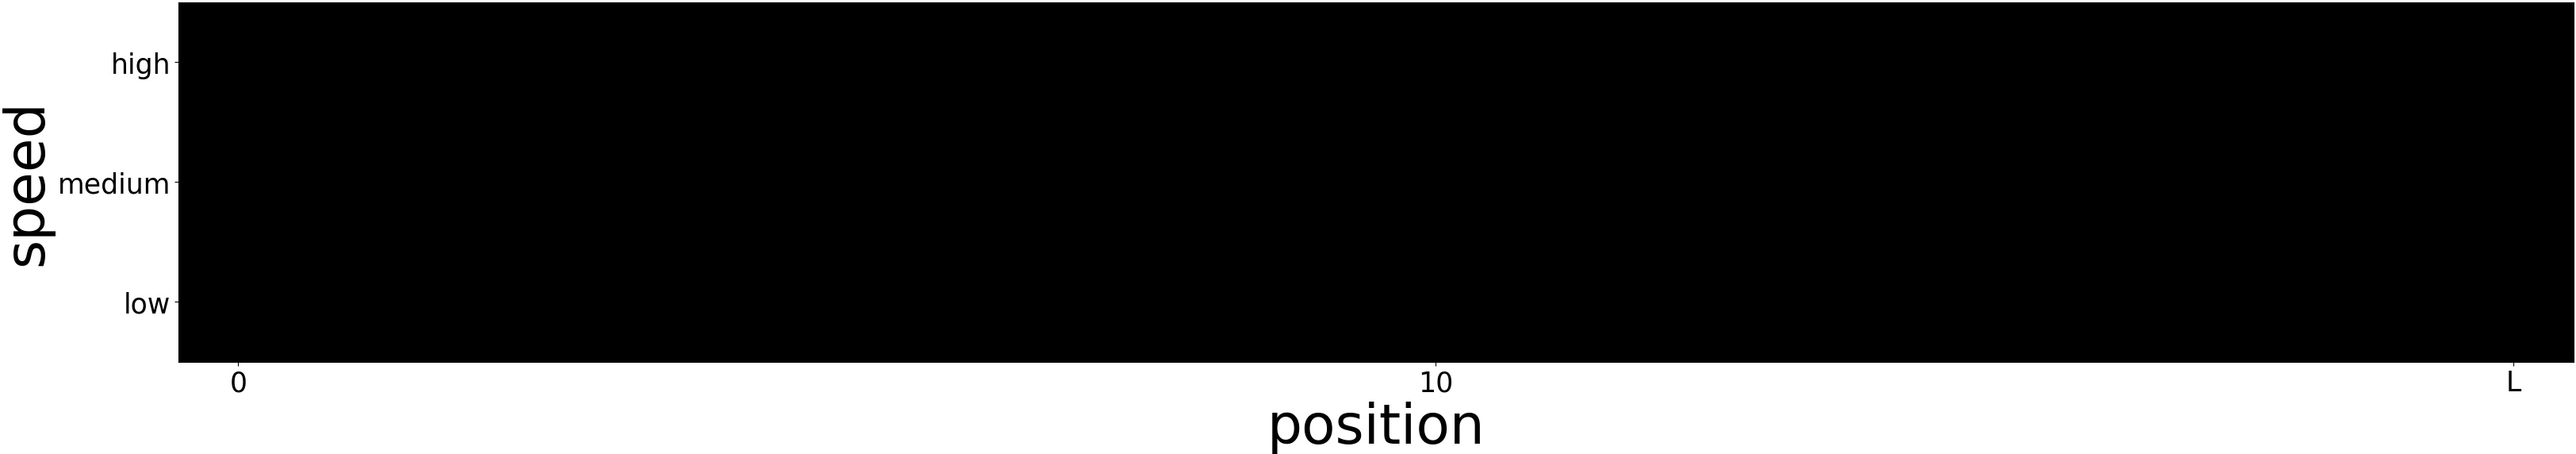
\includegraphics[scale=0.12]{img/value0.jpg}\\
\begin{block}{}
\centering
States values at iteration $0$, all the state values are equal to $0$
\end{block}

\end{frame}




\begin{frame}
\frametitle{State value function at different iterations}
\framesubtitle{the brighter the better the value}
\centering
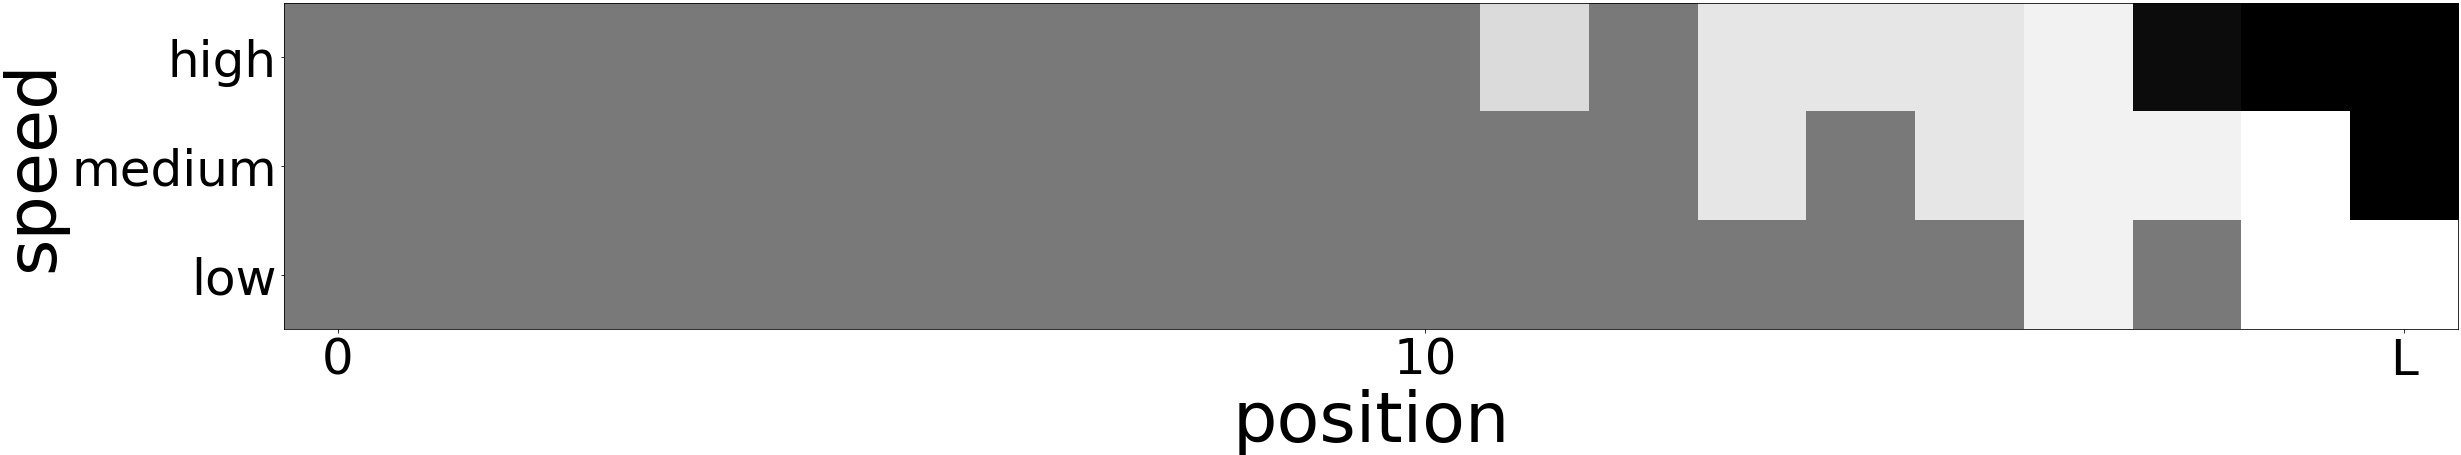
\includegraphics[scale=0.12]{img/value2.jpg}\\
\begin{block}{}
\centering
States values at iteration $2$ 
\end{block}
\end{frame}


\begin{frame}
\frametitle{State value function at different iterations}
\framesubtitle{the brighter the better the value}

\centering
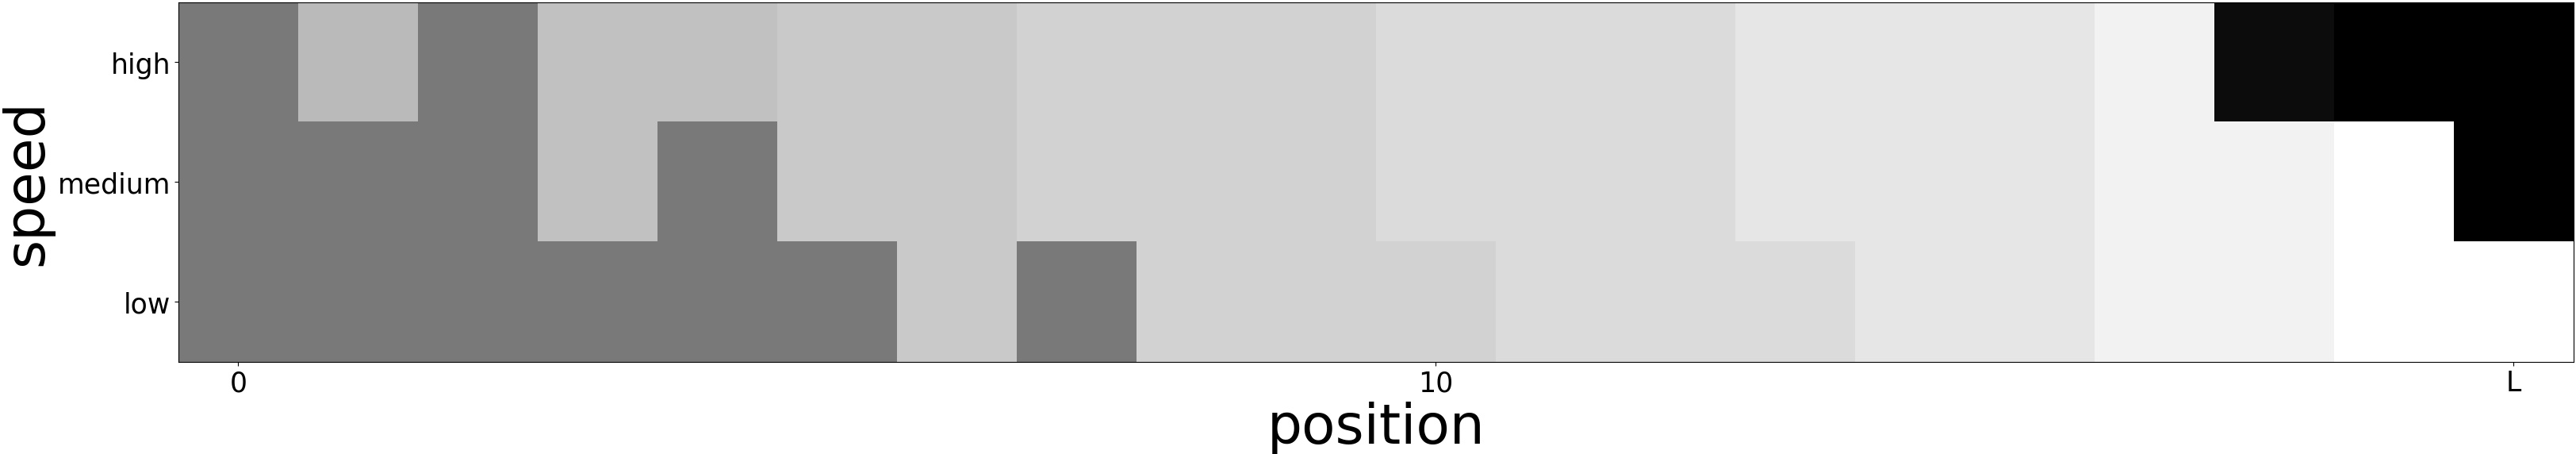
\includegraphics[scale=0.12]{img/value4.jpg}\\
\begin{block}{}
\centering
States values at iteration $4$ 
\end{block}
\end{frame}

\begin{frame}
\frametitle{State value function at different iterations}
\framesubtitle{the brighter the better the value}

\centering
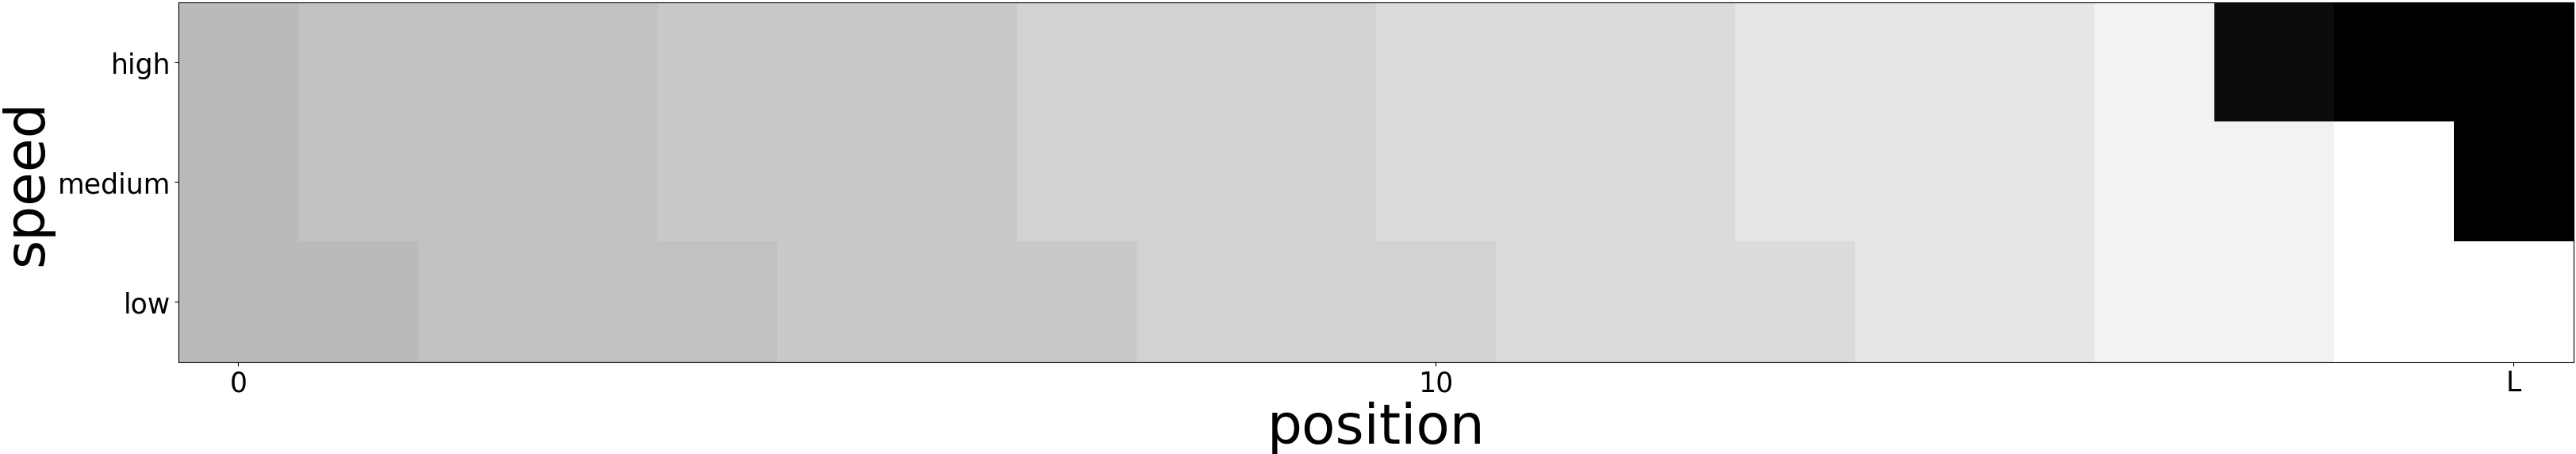
\includegraphics[scale=0.12]{img/value6.jpg}\\
\begin{block}{}
\centering
States values at iteration $6$ (where stable policy is attained)
\end{block}

\end{frame}



\begin{frame}
\frametitle{Results for deterministic actions}
\framesubtitle{One of the optimal trajectories}
\centering
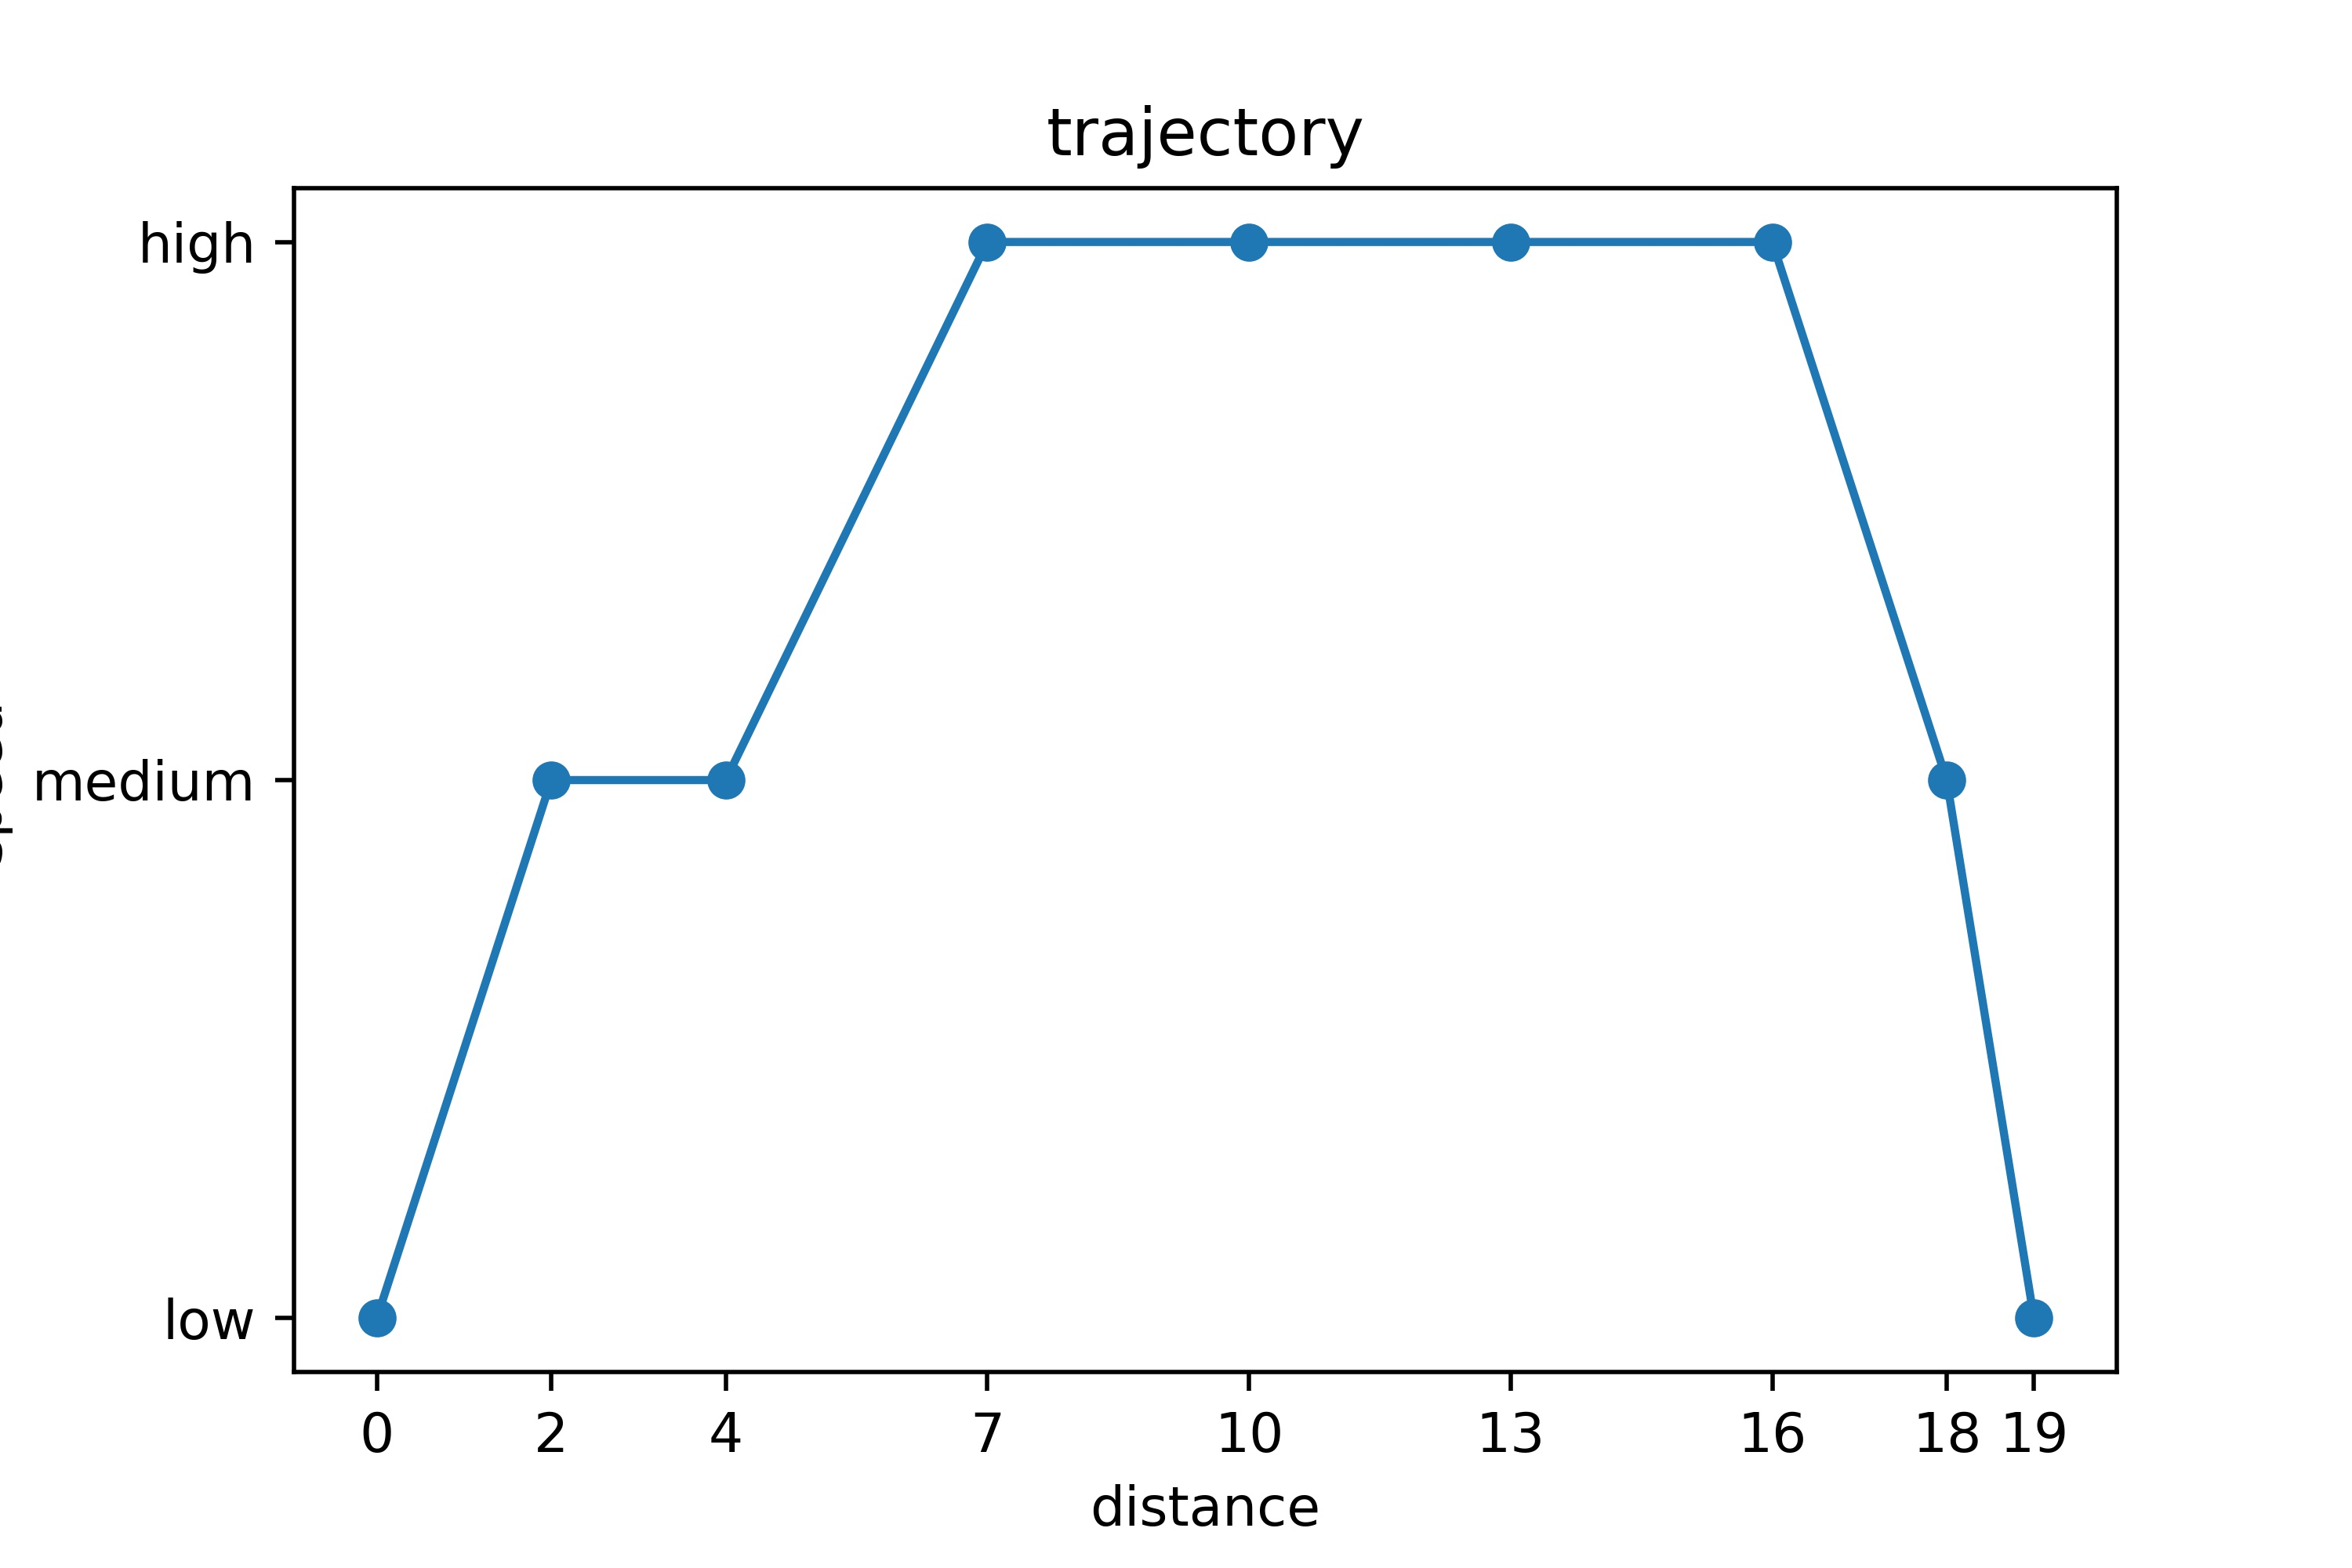
\includegraphics[scale=0.5]{img/trajectory.jpg}
\end{frame}


\begin{frame}
\frametitle{Deterministic actions are not really realistic}
\begin{columns}[c]
\column{1.5in}
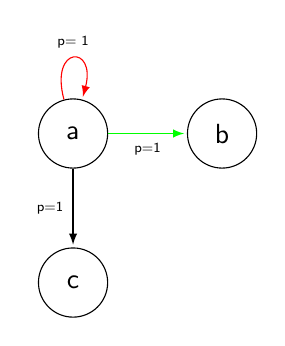
\begin{tikzpicture}[font=\sffamily]
         \node[state] (a) {a};
        \node[state] [right = 1 cm of a] (b) {b};
        \node[state] [below = 1 cm of a] (c) {c};
	\draw[every loop,
        auto=right,
        >=latex,
        draw=black,
        fill=black]
			(a) edge[loop above,draw = red] node{{\tiny p= 1}} (a)
			(a) edge[draw = green] node{{\tiny p=1}} (b)
			(a) edge[draw = black] node{{\tiny p=1}} (c);
    \end{tikzpicture}\\
\centering
Deterministic actions
\pause
\column{1.5in}
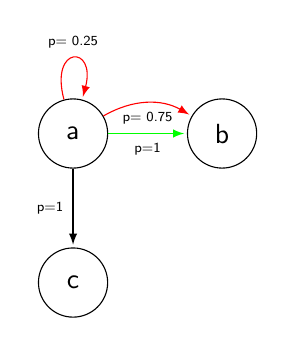
\begin{tikzpicture}[font=\sffamily]
         \node[state] (a) {a};
        \node[state] [right = 1 cm of a] (b) {b};
        \node[state] [below = 1 cm of a] (c) {c};
	\draw[every loop,
        auto=right,
        >=latex,
        draw=black,
        fill=black]
			(a) edge[loop above,draw = red] node{{\tiny p= 0.25}} (a)
			(a) edge[bend left,draw = red] node{{\tiny p= 0.75}} (b)
			(a) edge[draw = green] node{{\tiny p=1}} (b)
			(a) edge[draw = black] node{{\tiny p=1}} (c);
    \end{tikzpicture}\\
    \centering 
    Stochastic actions
    \end{columns}

\end{frame}



\begin{frame}
\begin{center}
\frametitle{Decelerating for decelerating being a stochastic action}

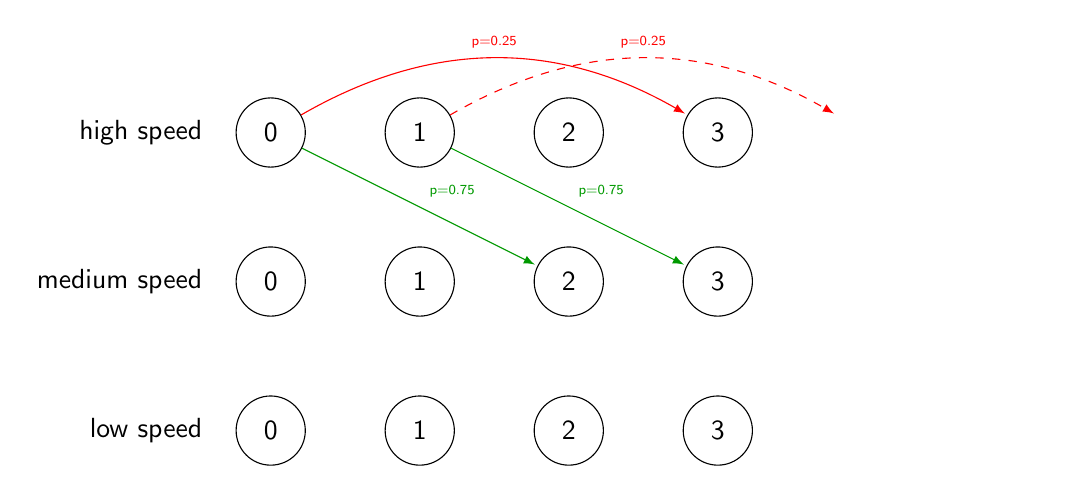
\begin{tikzpicture}[font=\sffamily]
    % Add the states
        %\node[state,draw=none] (d1) [left of=1] {};
        \node[state,text = black
              ] (h0) {0};
		\node[state,
			below=1 cm of h0,
			text = black
        	] (m0) {0};
		\node[state,
			below= 1 cm of m0,
        	text=black,
        	] (l0) {0};
         \node[state,
         	 right = 1 cm of h0,
             text = black
              ] (h1) {1};	
		\node[state,
			below=1 cm of h1,
        	text = black
        	] (m1) {1};
		\node[state,
			below= 1 cm of m1,
        	text=black,
        	] (l1) {1};
         \node[state,
         	right = 1 cm of h1,
         	text = black
              ] (h2) {2};	
		\node[state,
			below=1 cm of h2,
        	text = black,
        	] (m2) {2};
		\node[state,
		below= 1 cm of m2,
        	text=black,
        	] (l2) {2};
        \node[state,
        	right = 1 cm of h2,
        	text = black
             ] (h3) {3};	
		\node[state,
			below=1 cm of h3,
        	text=black
        	] (m3) {3};
		\node[state,
			below= 1 cm of m3,
        	text=black,
        	] (l3) {3};   	
		\node[state,draw=none] (d1) [right = 1 cm of l3] {};	
		\node[state,draw=none] (d2) [right = 1 cm of m3] {};
		\node[state,draw=none] (d3) [right = 1 cm of h3] {};
		\node[state,draw=none] (d4) [right = 1 cm of d3] {};
		\node[draw=none] (legend1) [left=0.3 cm of l0] {low speed};
		\node[draw=none] (legend2) [left = 0.3 cm of m0] {\textcolor{black}{medium speed}};
		\node[draw=none] (legend3) [left = 0.3 cm of h0] {\textcolor{black}{high speed}};
		        
       
	\draw[every loop,
        auto=left,
        >=latex,
        draw=black,
        fill=black]
			(h0) edge[ draw = black!40!green] node{{\textcolor{black!40!green}{\tiny p=0.75}}} (m2)
			(h1) edge[ draw = black!40!green] node{{\textcolor{black!40!green}{\tiny p=0.75}}} (m3);
			
	   \pause    \draw[every loop,
        auto=left,
        >=latex,
        draw=red,
        fill=red]

			(h0) edge[bend left]node{{\textcolor{red}{\tiny p=0.25}}} (h3)
			(h1) edge[bend left,dashed] node{{\textcolor{red}{\tiny p=0.25}}}(d3);
    \end{tikzpicture}
     \end{center}



\end{frame}

\begin{frame}
\frametitle{Results for stochastic actions}
\framesubtitle{state-value function at the end of the iterations
}
\centering
deterministic actions\\
\vspace{0.1cm}
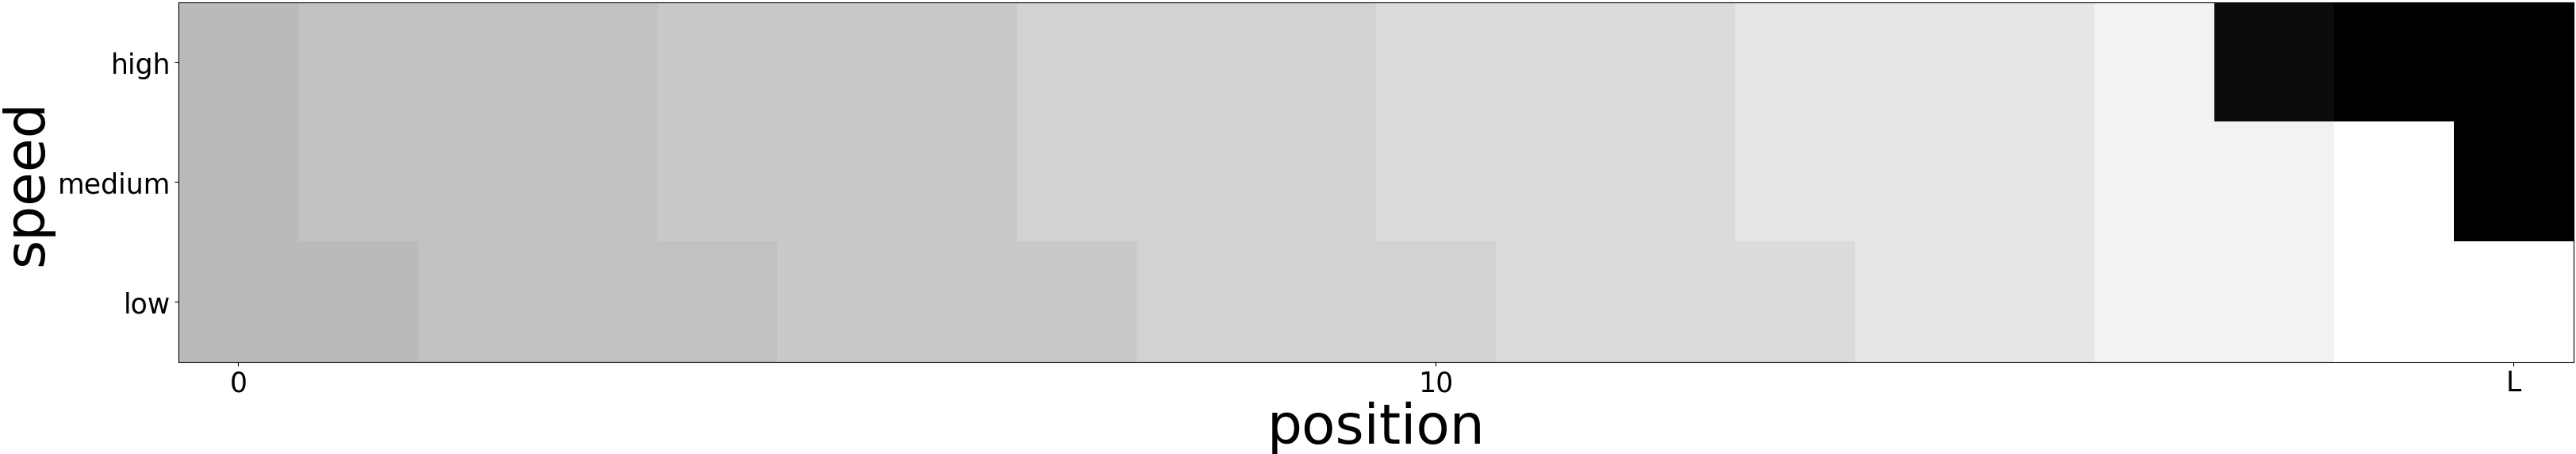
\includegraphics[scale=0.12]{img/value6.jpg}\\
\vspace{0.3cm}
stochastic actions\\
\vspace{0.1cm}
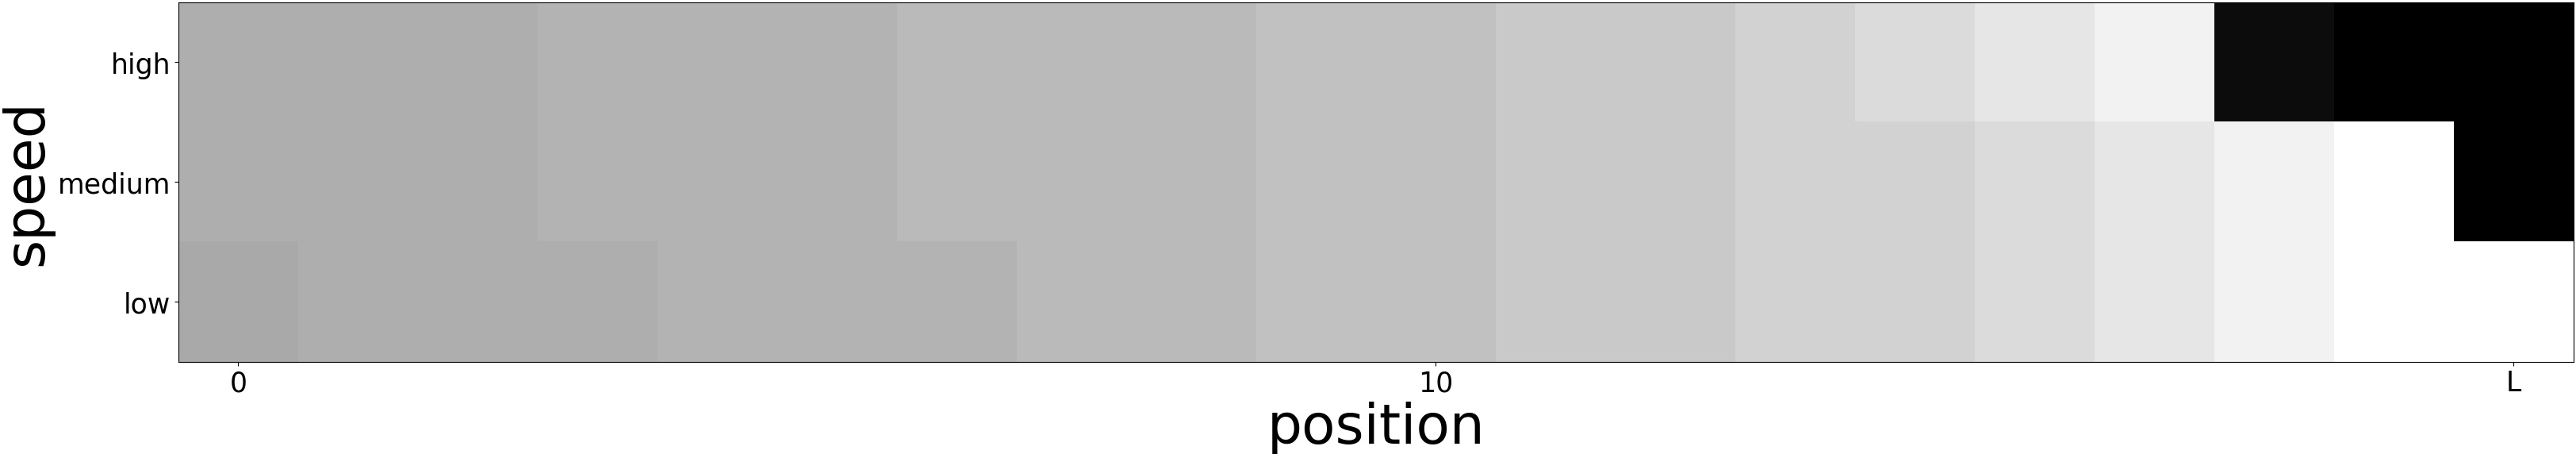
\includegraphics[scale=0.12]{img/state_values_sto.jpg}
\end{frame}

\begin{frame}
\frametitle{Results for stochastic actions}
\framesubtitle{decelerating  results in keeping the same speed with probability 1/4}
\centering
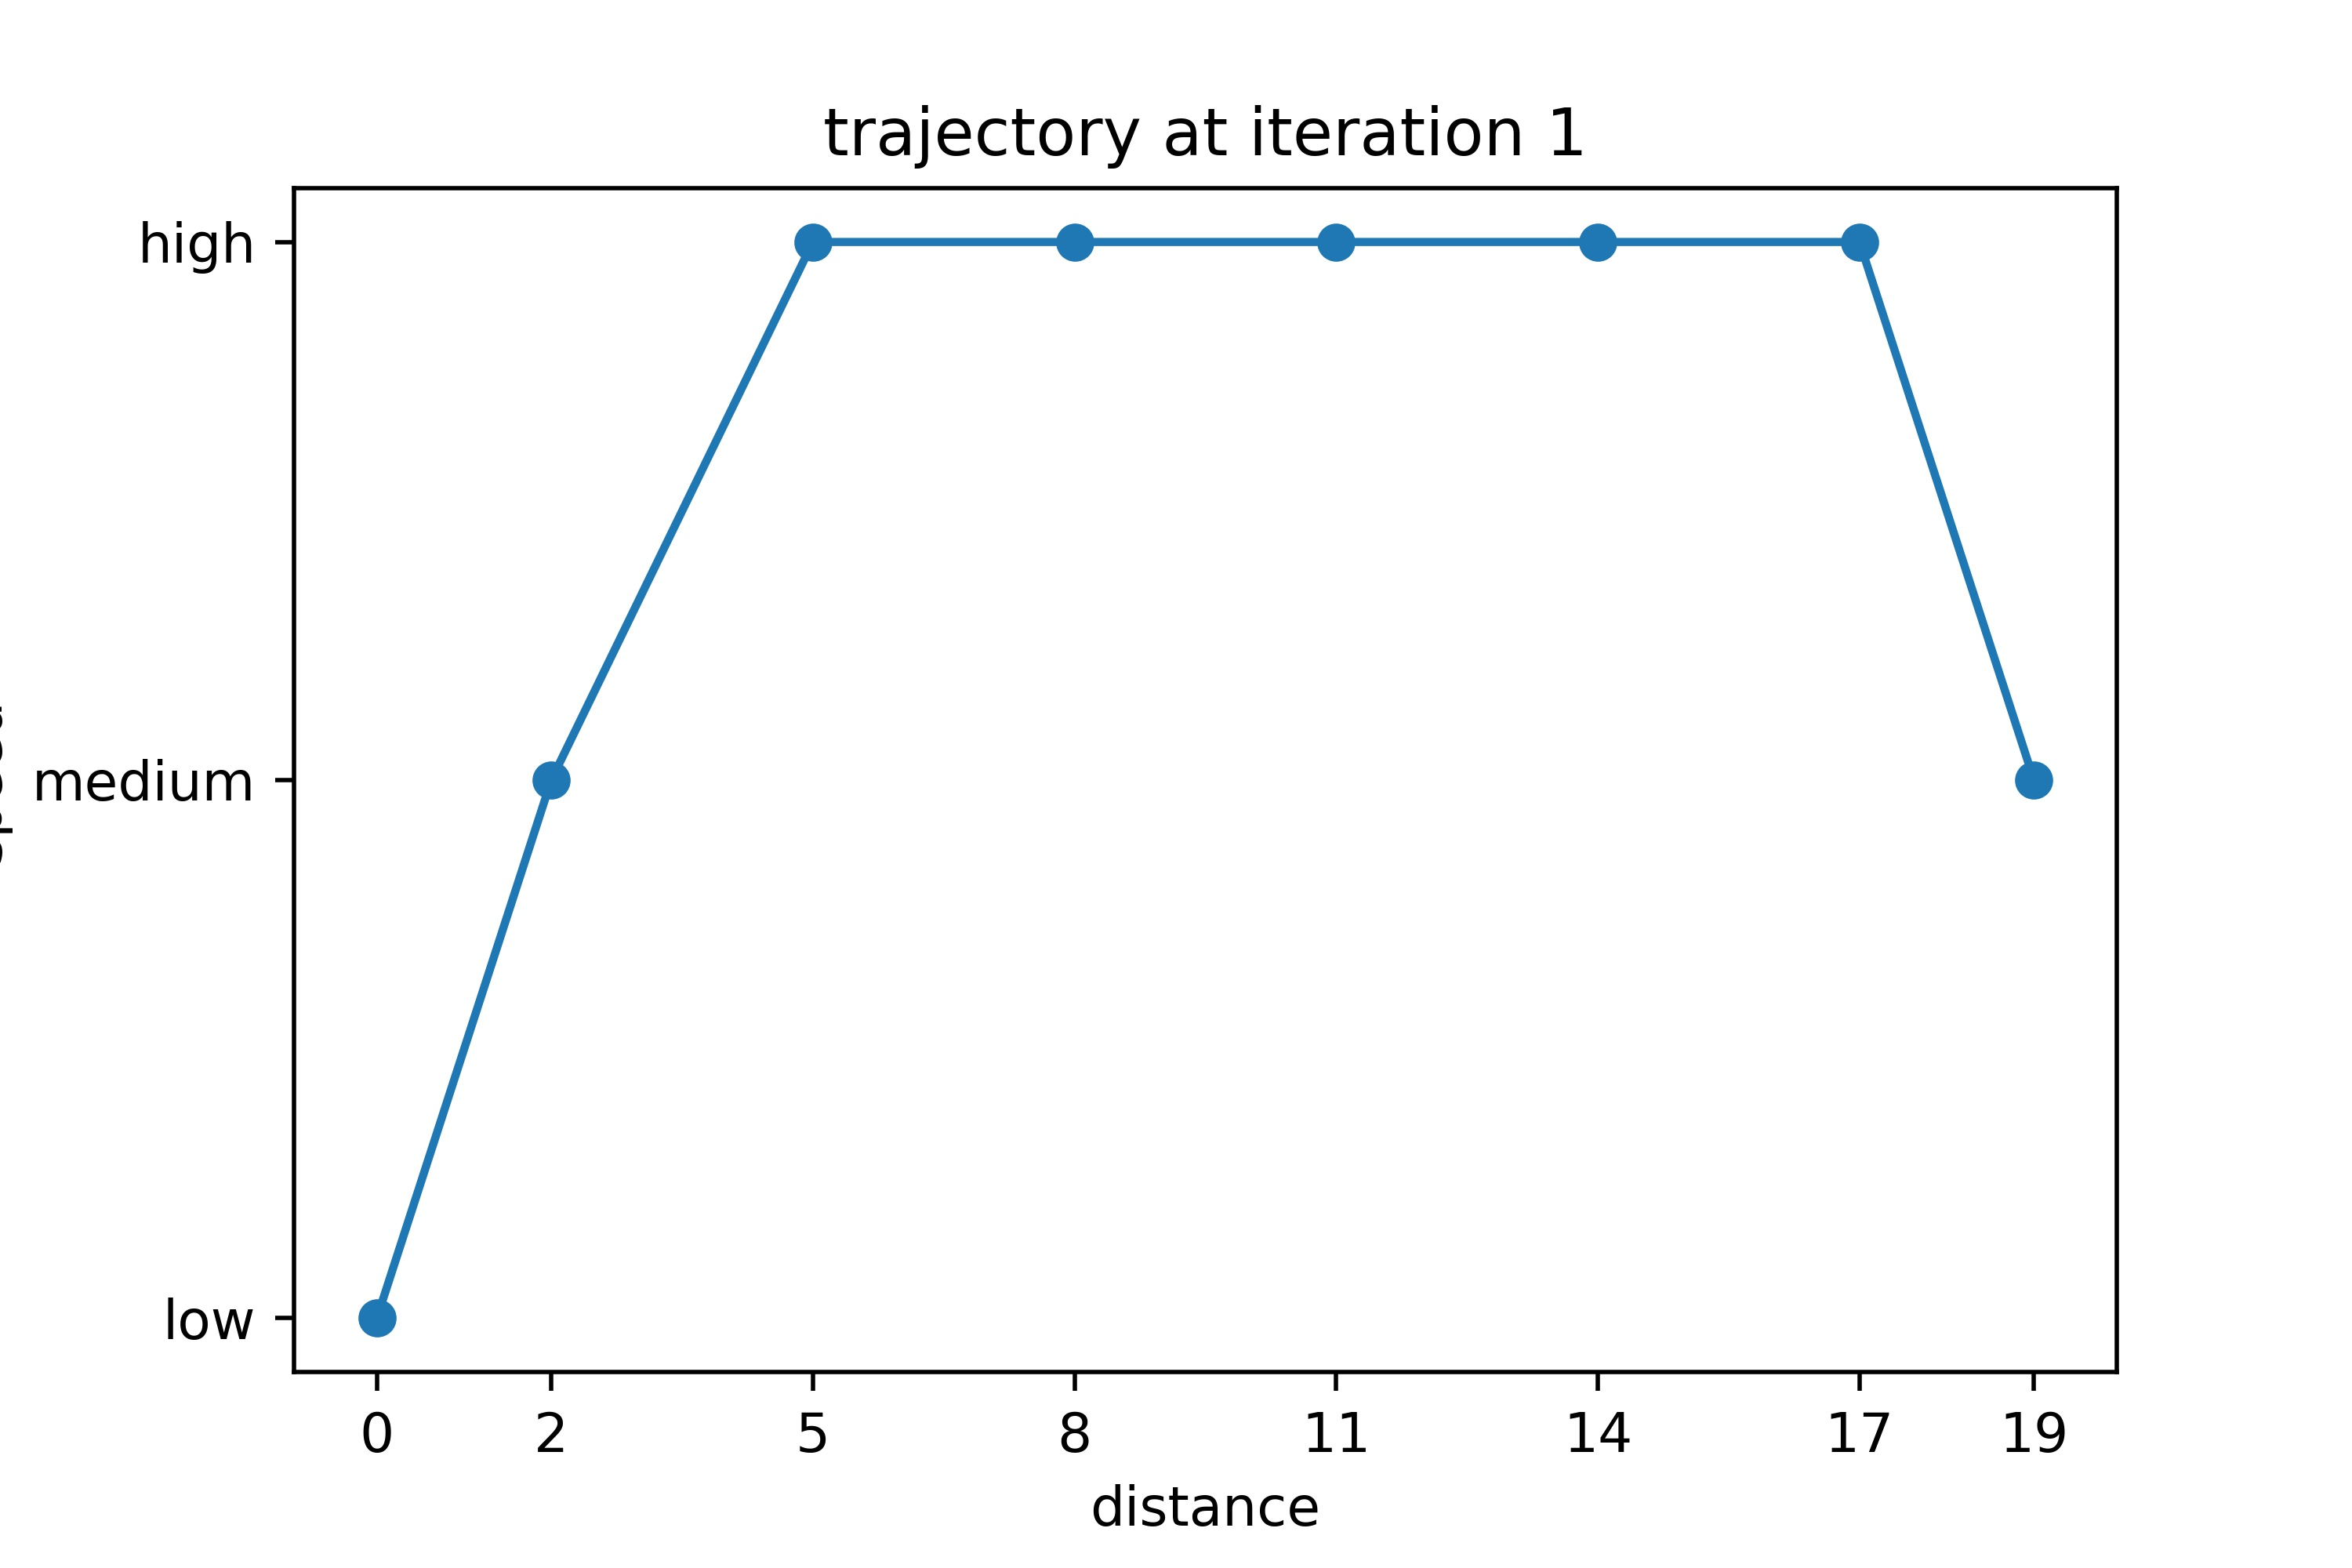
\includegraphics[scale=0.5]{img/trajectory1.jpg}
\end{frame}



\begin{frame}
\frametitle{Results for stochastic actions}
\framesubtitle{decelerating results results in keeping the same speed with probability 1/4}
\centering
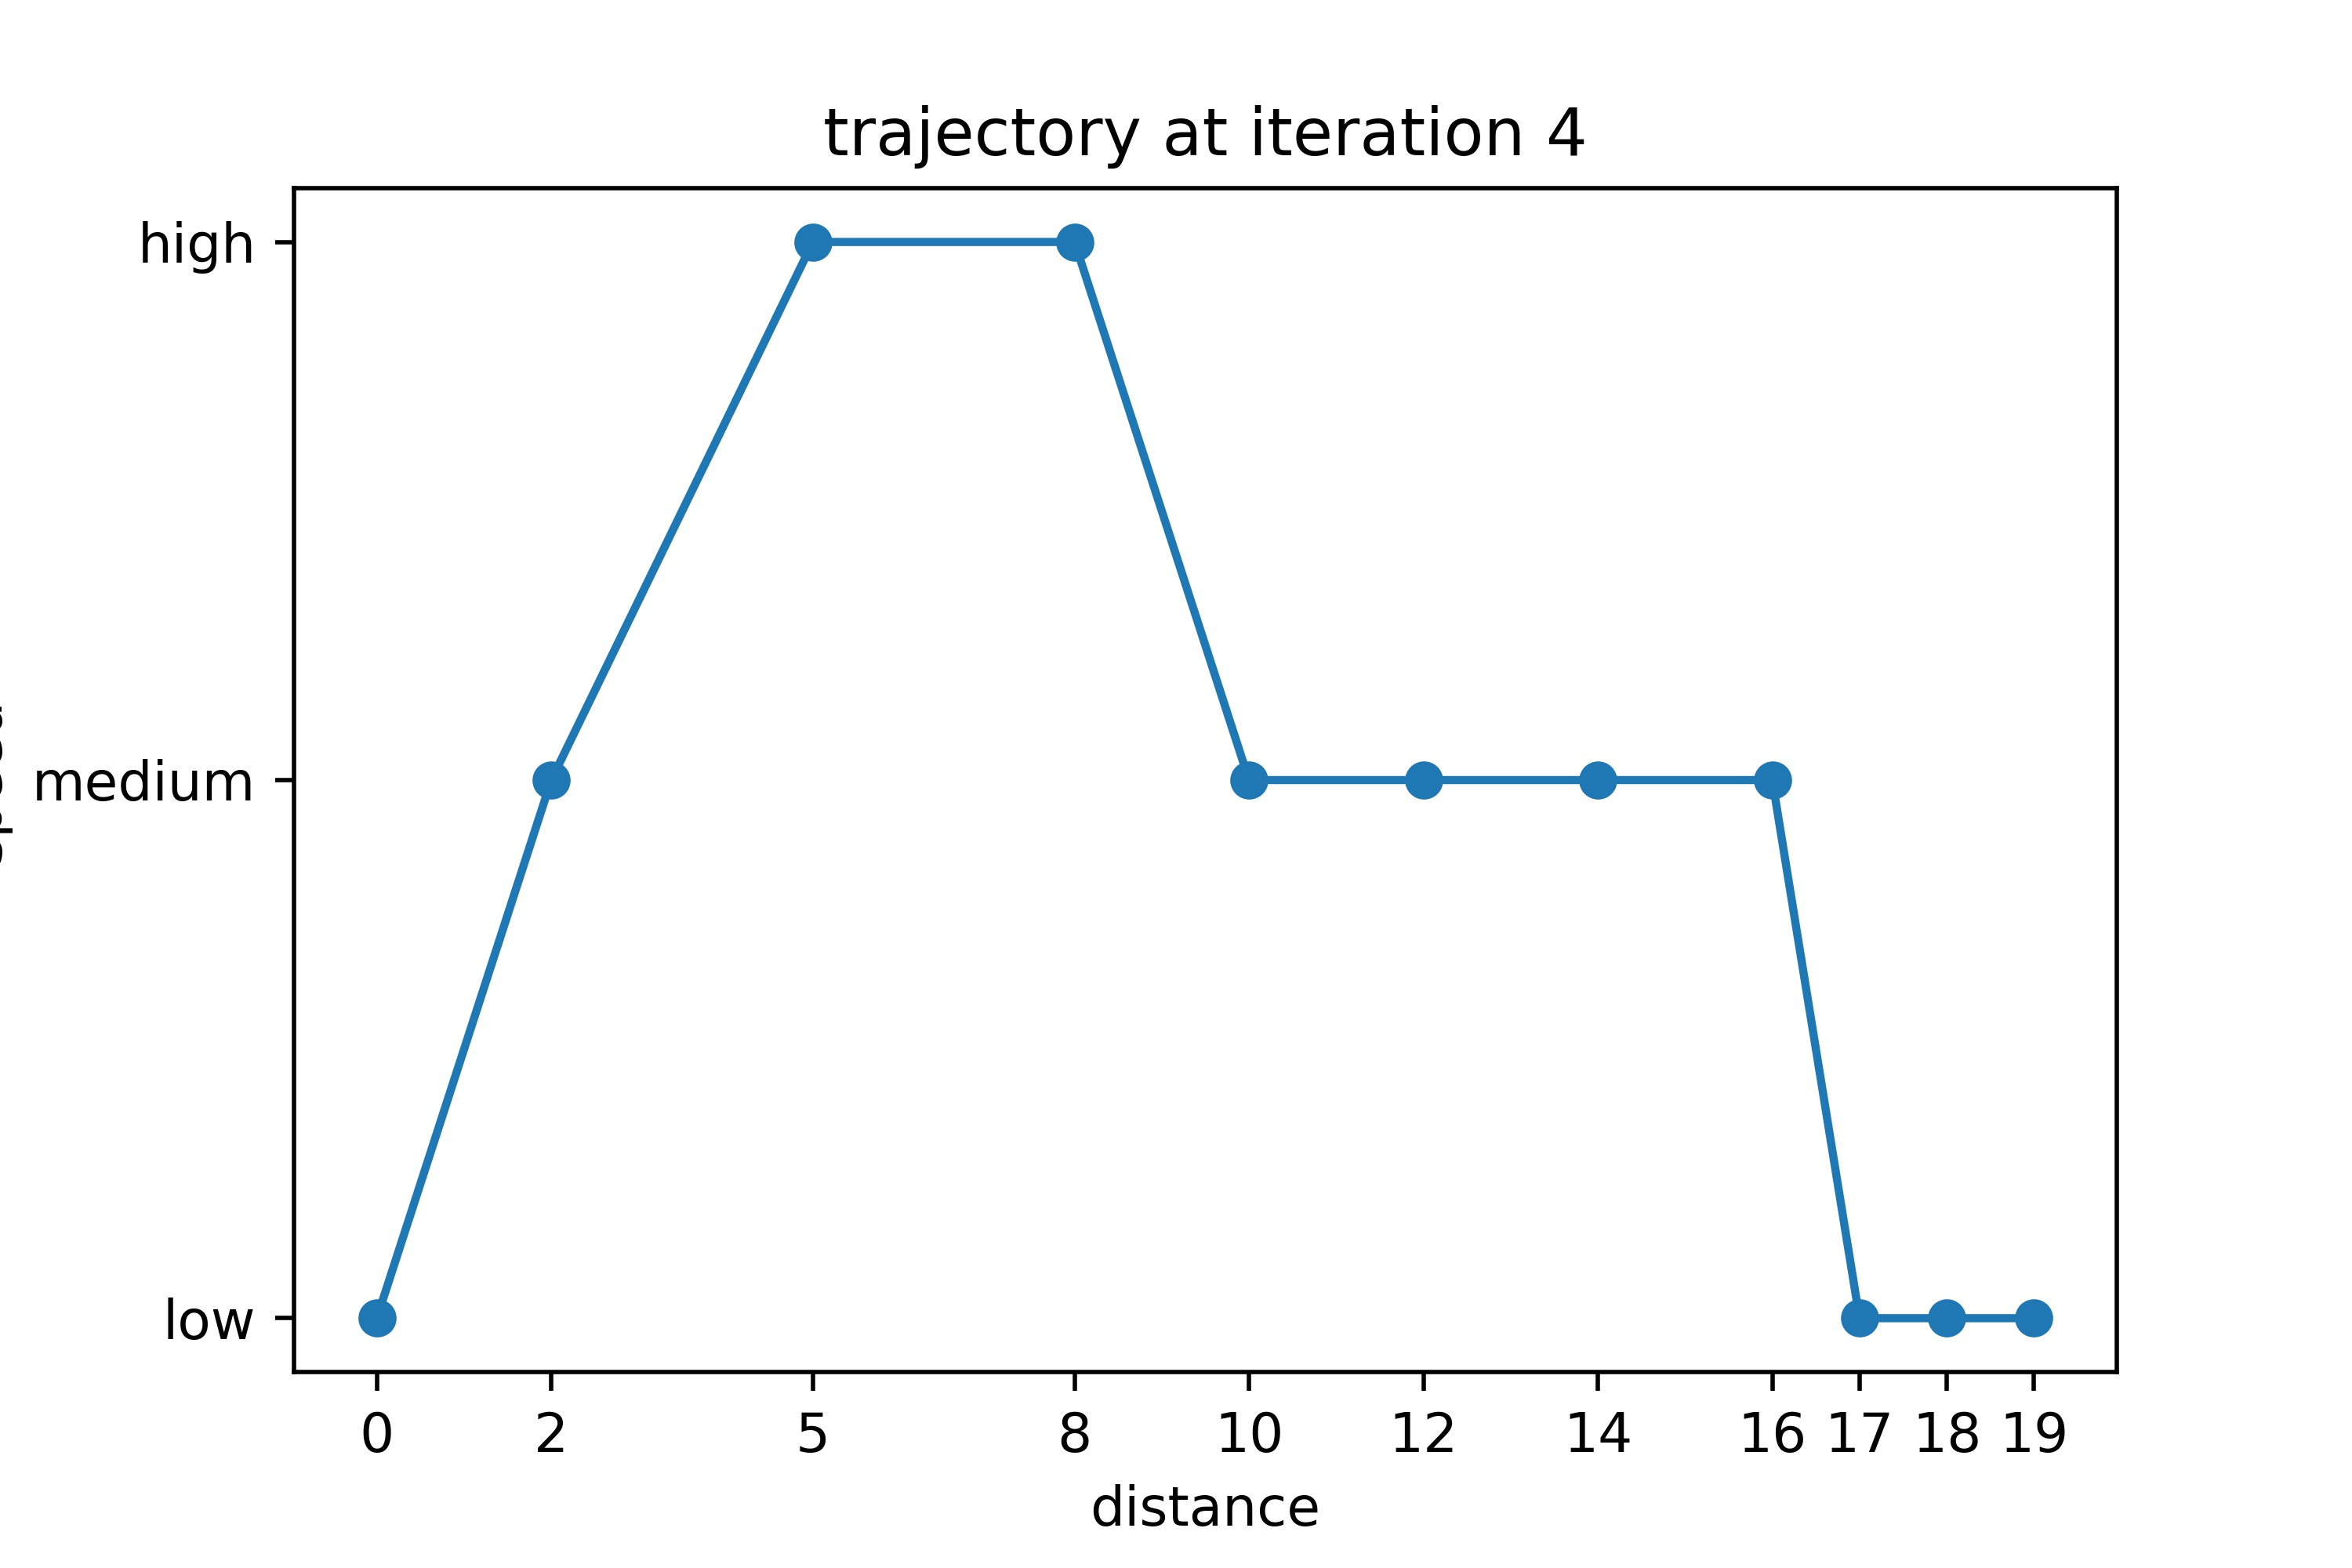
\includegraphics[scale=0.5]{img/trajectory4.jpg}\\
\centering
where stable policy is attained 
\end{frame}







\begin{frame}
\frametitle{Conclusion }
\begin{block}{}
\begin{itemize}
\item We introduced the theoretical framework: Reinforcement learning and Markov Decision Processes
\item We solved a simple problem where we know the model (the transition function in particular)
\end{itemize}
\end{block}
\end{frame}



\begin{frame}
\frametitle{What's next ? }



\begin{block}{already working on}
\begin{itemize}
\item Add the traffic light into this setting
\item Find the distance from the robot's camera to the traffic light
\item getting data from the robot 
\end{itemize}
\end{block}

\begin{block}{In a not so distant future}
\begin{itemize}
\item Explore other algorithms and compare them : Monte-Carlo methods, temporal difference learning, Q learning, Expected Sarsa$\ldots$
\item Neuro-dynamic programming ?
\end{itemize}
\end{block}

\pause
\begin{block}{Ultimately}
Implement everything on the robot ... \pause and pray that everything works well
\end{block}

\end{frame}




\end{document}
